\documentclass[11pt,a4paper]{article}

\usepackage[margin=0.75in]{geometry}
\usepackage{graphicx}
\usepackage{amsmath}
\usepackage{amssymb}
\usepackage{fancyhdr}
\usepackage{color}
\usepackage{url}

\pagestyle{fancy}
\fancyhf{}
\lhead{\small \textcolor{gray}{MiniBass: Technical Report}}
\rhead{\small \textcolor{gray}{$10 \times 12\text{ m}$ Venue Acoustic Optimization}}
\cfoot{\thepage}

\definecolor{navy}{rgb}{0.0, 0.2, 0.4}
\definecolor{darkred}{rgb}{0.7, 0.1, 0.1}
\definecolor{darkgreen}{rgb}{0.1, 0.5, 0.1}
\definecolor{darkgray}{rgb}{0.3, 0.3, 0.3}
\definecolor{gray}{rgb}{0.5, 0.5, 0.5}

\newenvironment{proof}{\noindent\textbf{Proof.}}{\hfill$\blacksquare$\vspace{0.5em}\par}

\title{\vspace{-1.5cm}\textbf{\LARGE MiniBass: Optimization and Synthesis of Low-Frequency Sound Fields in a $10 \times 12\text{ m}$ Performance Venue}\\[0.3em]
\Large Discrete Modal Superposition, Active Phase DSP, Baseline Comparisons, and Physical Uncertainty}
\author{}
\date{November 2026}

\begin{document}

\maketitle

\begin{abstract}
\noindent Low-frequency sound reproduction ($20\text{--}200\text{ Hz}$) in enclosed rectangular acoustic spaces is corrupted by standing wave modal resonances, creating severe spatial sound pressure level (SPL) variance across audience seats. This technical report presents the physical derivation, algorithmic implementation, empirical execution, comparative baselines, and formal mathematical analysis of an idealized multi-subwoofer bass reproduction system for a $10.0 \times 12.0 \times 2.8\text{ m}$ performance hall ($V = 336\text{ m}^3$, $T_{60} = 0.45\text{ s}$). The layout incorporates a centered front stage ($8.0 \times 2.0\text{ m}$) along the short wall ($y = 0\text{ m}$) and an audience listening zone spanning $x \in [0.2, 9.8]\text{ m}$ and $y \in [2.2, 11.8]\text{ m}$, establishing an exact $0.2\text{ m}$ perimeter margin from all walls and the stage front. Across an 80-seat audience grid and 95 refined discrete frequencies, a discrete pruned beam-search optimizer evaluated $104,145$ physical configurations, identifying a best-found 4-box asymmetric front-stage array ($x = 3.39, 4.46, 7.68, 8.75\text{ m}$) with heterogeneous 10-inch ported enclosures and differentiated active DSP controls (2 ms delay on stage-left, 120 Hz lowpass on stage-right). 

The best-found design achieves an RMS flatness error of $6.25\text{ dB}$, an audience spatial mean of $79.44\text{ dB SPL}$ (though individual seats exhibit a $\pm 1$ standard deviation corridor of roughly $\pm 5\text{ dB}$), and a tolerance corridor pass rate of $39.28\%$ ($2,985 / 7,600$ seat-frequency pairs within $\pm 3\text{ dB}$ of the $80.0\text{ dB SPL}$ target). Comparative baselines show that a single corner subwoofer yields $9.33\text{ dB}$ RMS error ($16.11\text{ dB}$ worst-seat error), while a symmetric 4-subwoofer array without DSP yields $6.99\text{ dB}$ RMS error ($11.52\text{ dB}$ worst-seat error). The asymmetric layout alone reduces RMS error to $6.59\text{ dB}$, and active DSP achieves $6.25\text{ dB}$ ($9.97\text{ dB}$ worst-seat error). Validation on 40 held-out off-grid listener positions demonstrates physical generalization with $6.16\text{ dB}$ RMS error. A 256-sample environmental and physical uncertainty Monte Carlo analysis (perturbing sound speed $\pm 2\%$, reverberation time $\pm 10\%$, speaker placement $\sigma = 5\text{ cm}$, seat position $\sigma = 10\text{ cm}$, and driver parameters $\pm 5\%$) confirms parameter robustness, with a 90\% confidence interval for RMS error of $[6.18, 6.40]\text{ dB}$. Formal Lean 4 meta-theorems and empirical single-frequency projections confirm that a strict 95\% full-band coverage target is mathematically infeasible under the discrete hardware catalog, establishing that multi-seat optimization must target minimax and RMS flatness rather than binary all-seat acceptance gates.
\end{abstract}

\vspace{0.5em}
\hrule
\vspace{1.0em}

\section{Aim and Operational Context}

The primary engineering objective of this investigation is the numerical optimization, physical simulation, and empirical evaluation of a multi-source low-frequency sound reinforcement system within a designated $10.0 \times 12.0 \times 2.8\text{ m}$ performance venue. 

In traditional single-subwoofer sound systems, room boundary reflections cause constructive and destructive interference, creating severe resonant peaks ($+12\text{ to }+18\text{ dB}$) and deep non-minimum-phase interference notches ($-20\text{ to }-30\text{ dB}$) that cannot be corrected by global equalization. The objective is to evaluate whether a multi-transducer array constrained entirely to the front stage boundary can mitigate audience seat-to-seat variance, reduce room-wide RMS response error relative to an $80.0\text{ dB SPL}$ ($0.20\text{ Pa RMS}$) target corridor, and improve worst-seat acoustic consistency across the $20\text{--}200\text{ Hz}$ band.

\subsection{Venue Specification and Geometric Boundaries}
\begin{itemize}
    \item \textbf{Room Dimensions:} Lengths $L_x = 10.0\text{ m}$ (short edge), $L_y = 12.0\text{ m}$ (long edge), and height $L_z = 2.8\text{ m}$. Enclosed volume $V = 336.0\text{ m}^3$. Reverberation time $T_{60} = 0.45\text{ s}$ across all bass modes, modeling standard commercial acoustic boundary absorption.
    \item \textbf{Front Stage Geometry:} The stage is located on the short edge at $y = 0\text{ m}$, centered along the $x$-axis, with dimensions $8.0\text{ m}$ (width) $\times 2.0\text{ m}$ (depth). In Cartesian coordinates, the stage occupies $x \in [1.0, 9.0]\text{ m}$ and $y \in [0.0, 2.0]\text{ m}$.
    \item \textbf{Subwoofer Placement Menu:} Candidate cabinet centers are restricted to 8 floor-level positions along the stage front line ($y = 1.78\text{ m}$, elevation $z = 0.40\text{ m}$), spanning $x \in [1.25, 8.75]\text{ m}$ in uniform linear increments ($\Delta x \approx 1.07\text{ m}$).
    \item \textbf{Audience Seating Footprint:} Constrained strictly by a \textbf{$0.2\text{ m}$ margin} from the stage front and all room boundary walls:
    \begin{equation}
        \mathcal{X}_{\text{seating}} = [0.2, 9.8]\text{ m} \quad (\text{width } 9.6\text{ m}), \qquad \mathcal{Y}_{\text{seating}} = [2.2, 11.8]\text{ m} \quad (\text{depth } 9.6\text{ m})
    \end{equation}
    defining an exact $9.6 \times 9.6\text{ m}$ square listening area.
    \item \textbf{In-Sample Audience Receivers:} A regular grid of $R = 80$ listener seats ($10\text{ columns} \times 8\text{ rows}$), cell-centered within the seating footprint at standard seated ear height $z = 1.10\text{ m}$. Lateral column pitch is $\Delta x = 0.96\text{ m}$ ($x_i \in [0.68, 9.32]\text{ m}$); longitudinal row pitch is $\Delta y = 1.20\text{ m}$ ($y_j \in [2.80, 11.20]\text{ m}$).
    \item \textbf{Held-Out Validation Receivers:} A secondary set of 40 off-grid evaluation coordinates placed strictly between in-sample rows and columns ($x \in [0.68, 9.32]\text{ m}, y \in [2.80, 11.20]\text{ m}$, at $z = 1.10\text{ m}$), used exclusively for blind generalization auditing.
\end{itemize}

\subsection{Physical Wave Considerations: Nyquist Sampling and Schroeder Transition}
Two foundational physical boundaries govern acoustic modeling in this enclosure:
\begin{enumerate}
    \item \textbf{Spatial Sampling and Nyquist Cutoff:} The half-wavelength at $200\text{ Hz}$ is $\lambda / 2 = c / (2 f) = 343 / 400 = 0.8575\text{ m}$. With longitudinal row spacing $\Delta y = 1.20\text{ m}$, the spatial Nyquist frequency along $y$ is:
    \begin{equation}
        f_{\text{Nyq}, y} = \frac{c}{2 \Delta y} = \frac{343}{2 \times 1.20} \approx 142.9\text{ Hz}
    \end{equation}
    Along the transverse axis with column spacing $\Delta x = 0.96\text{ m}$, the spatial Nyquist frequency is $f_{\text{Nyq}, x} = c / (2 \Delta x) \approx 178.6\text{ Hz}$. Consequently, while the 80-seat grid satisfies spatial Nyquist criteria below $142.9\text{ Hz}$, spatial aliasing occurs on the discrete seat grid between $143\text{ Hz}$ and $200\text{ Hz}$. Continuous wave field evaluations require dense evaluation grids rather than seat-sampled approximations.
    \item \textbf{Schroeder Frequency and Modal Regimes:} In this $336\text{ m}^3$ enclosure with $T_{60} = 0.45\text{ s}$, the classical Schroeder cutoff frequency is:
    \begin{equation}
        f_s \approx 2000 \sqrt{\frac{T_{60}}{V}} = 2000 \sqrt{\frac{0.45}{336}} \approx 73.2\text{ Hz}
    \end{equation}
    Below $f_s \approx 73.2\text{ Hz}$, the acoustic response is dominated by discrete, isolated standing wave modes with low modal overlap ($M < 3$). Above $73.2\text{ Hz}$, modal overlap increases rapidly ($M > 3$), transitioning into a dense statistical multimodal interference regime. Thus, acoustic behavior from $100\text{--}200\text{ Hz}$ is governed by overlapping modal wave fields rather than isolated sparse room modes.
\end{enumerate}

\section{Base Papers ($\ge 2025$) and Exact Project Inferences}

To ground the methodology in recent peer-reviewed acoustics research, the optimization engine incorporates concepts from literature published in 2025:

\subsection{Base Paper 1: Modal-Domain Placement Optimization}
\noindent \textbf{Citation:} Xin Wen, Haijun Wu, Dianlong Chen, and Weikang Jiang, ``Optimizing loudspeaker placement based on modal domain analysis for multizone sound field reproduction,'' \textit{Applied Acoustics}, vol. 240, p. 110904, 2025. DOI: \url{https://doi.org/10.1016/j.apacoust.2025.110904}.

\noindent \textbf{Exact Inference Used in MiniBass:}
Wen et al. demonstrate that optimizing secondary source positions directly in the space-time domain leads to ill-conditioned nonlinear problems. Instead, projecting acoustic transfer paths into orthogonal modal eigenfunctions decouples cavity geometry from source transducer dynamics. 
In MiniBass, this principle is operationalized by separating the rectangular transfer matrix into 3D eigenfunctions $\psi_{\mathbf{n}}(\mathbf{x})$ and modal frequency responses, precomputing source volume velocities $q_a(\omega)$ across discrete enclosure-driver-DSP atoms, and evaluating candidate combinations via linear tensor superposition:
\begin{equation}
    p(r, k) = \sum_{s \in S} H(r, \operatorname{pos}(s), k) q_s(k)
\end{equation}

\subsection{Base Paper 2: Transducer Parameter Tolerances and Sensitivity}
\noindent \textbf{Citation:} Shang Zhao, Haoxin Ruan, Zhibin Lin, and Jing Lu, ``Orthogonal loudspeaker matching for stable and accurate multizone sound field reproduction,'' \textit{Applied Acoustics}, vol. 231, p. 110507, 2025. DOI: \url{https://doi.org/10.1016/j.apacoust.2025.110507}.

\noindent \textbf{Exact Inference Used in MiniBass:}
Zhao et al. analyze the sensitivity of multi-channel loudspeaker arrays to physical tolerances, establishing that small perturbations in transducer parameters can degrade active cancellation. While initial studies examined driver voice-coil tolerances, physical room variations (speed of sound $c$, boundary absorption $T_{60}$, and transducer/seat positioning) dominate low-frequency transfer in enclosed spaces. MiniBass implements a 256-sample physical uncertainty audit that perturbs environmental sound speed ($\pm 2\%$), room damping ($\pm 10\%$), subwoofer positioning ($\sigma = 5\text{ cm}$), and listener head coordinates ($\sigma = 10\text{ cm}$).

\subsection{Base Paper 3: Physical Wave Fields vs. Interpolation Artifacts}
\noindent \textbf{Citation:} Yidong Liu, Kean Chen, Lei Yang, Jianfeng Luo, and Tong Gao, ``Secondary source placement optimization for sound field reproduction assisted by sound field interpolation,'' \textit{Applied Acoustics}, vol. 240, p. 110978, 2025. DOI: \url{https://doi.org/10.1016/j.apacoust.2025.110978}.

\noindent \textbf{Exact Inference Used in MiniBass:}
Liu et al. demonstrate that mathematical spatial interpolation (e.g., nearest-neighbor or polynomial extrapolation) across discrete receiver points introduces unphysical artifacts near room boundaries and violates the Helmholtz wave equation. 
In MiniBass, all 2D spatial acoustic error heatmaps and modal slices are computed by evaluating the exact closed-form 3D Helmholtz modal Green's function across dense coordinate grids ($40 \times 48$ and $100 \times 120$) directly from complex source flows $q_s(\omega)$, eliminating Voronoi extrapolation artifacts.

\section{Systematic Literature Review}

Table~\ref{tab:lit_review} and the following catalog review 10 foundational publications that inform the design of the MiniBass framework.

\begin{table}[h!]
\centering
\small
\renewcommand{\arraystretch}{1.15}
\caption{Systematic Literature Review: Methodological Domain and Exact Project Inference}
\label{tab:lit_review}
\resizebox{\textwidth}{!}{%
\begin{tabular}{|l|l|c|p{7.0cm}|}
\hline
\textbf{Inference Domain} & \textbf{Key Reference} & \textbf{Year} & \textbf{Exact Inference Used in MiniBass} \\ \hline
Discrete Placement & Wen et al. & 2025 & Modal eigenfunction projection \& atom tensor precomputation \\
Sensitivity & Zhao et al. & 2025 & Sensitivity to physical tolerances; environmental Monte Carlo \\
Wave Modeling & Liu et al. & 2025 & Elimination of Voronoi extrapolation; direct modal Green's functions \\
Heuristic Search & Zhou et al. & 2025 & Layered expansion \& bounded beam pruning \\
Sampling Bounds & Cadavid et al. & 2025 & Receiver density analysis; spatial Nyquist limits \\
Active Absorption & Laborie et al. & 2023 & Front emitter array + delayed boundary sink to cancel reflections \\
Spatial Flatness & Toole & 2018 & Multi-seat spatial consistency \& seat-to-seat variance metric \\
Mode Cancellation & Welti \& Devantier & 2006 & Multi-subwoofer symmetry; active DSP breaks shared nulls \\
Modal Diversity & Geddes & 2006 & Asymmetric spatial placement decorrelates transverse room modes \\
Transducer Physics & Small & 1973 & Coupled Thiele-Small electromechanical matrix equations \\
\hline
\end{tabular}%
}
\end{table}

\begin{enumerate}
    \item 
    \begin{itemize}
        \item \textbf{Inference Title:} Modal-Domain Decomposition \& Discrete Atom Precomputation
        \item \textbf{Paper:} \textit{Optimizing loudspeaker placement based on modal domain analysis for multizone sound field reproduction}, Applied Acoustics, vol. 240, p. 110904, 2025.
        \item \textbf{Authors:} Xin Wen, Haijun Wu, Dianlong Chen, and Weikang Jiang
        \item \textbf{Exact Inference Used:} Decoupling cavity modal eigenfunctions from transducer electromechanics to precalculate complex pressure tensors, accelerating multi-source combinatorial evaluation.
    \end{itemize}

    \item 
    \begin{itemize}
        \item \textbf{Inference Title:} Physical Tolerance Sensitivity \& Environmental Perturbations
        \item \textbf{Paper:} \textit{Orthogonal loudspeaker matching for stable and accurate multizone sound field reproduction}, Applied Acoustics, vol. 231, p. 110507, 2025.
        \item \textbf{Authors:} Shang Zhao, Haoxin Ruan, Zhibin Lin, and Jing Lu
        \item \textbf{Exact Inference Used:} Identifies array degradation under component variations; implemented via Monte Carlo perturbation of room temperature/sound speed, boundary absorption, and physical locations.
    \end{itemize}

    \item 
    \begin{itemize}
        \item \textbf{Inference Title:} First-Principles Wave Modeling \& Interpolation Artifact Elimination
        \item \textbf{Paper:} \textit{Secondary source placement optimization for sound field reproduction assisted by sound field interpolation}, Applied Acoustics, vol. 240, p. 110978, 2025.
        \item \textbf{Authors:} Yidong Liu, Kean Chen, Lei Yang, Jianfeng Luo, and Tong Gao
        \item \textbf{Exact Inference Used:} Replaced numerical nearest-neighbor spatial extrapolation with first-principles 3D Helmholtz modal Green's function evaluations across dense room grids, eliminating artificial Voronoi boundaries.
    \end{itemize}

    \item 
    \begin{itemize}
        \item \textbf{Inference Title:} Layered Beam Search \& Stepwise Candidate Pruning
        \item \textbf{Paper:} \textit{Stepwise-based optimizing approaches for arrangements of loudspeaker in multi-zone sound field reproduction}, Acoustical Science and Technology, vol. 46, no. 1, pp. 11--21, 2025.
        \item \textbf{Authors:} Tong Zhou, Kazuya Yasueda, Ghada Bouattour, Anthimos Georgiadis, and Akitoshi Kataoka
        \item \textbf{Exact Inference Used:} Implemented layered discrete expansion ($d = 1, 2, 3, 4$) combined with bounded beam retention ($W=32$) and canonical ordering, preventing combinatorial explosion while avoiding greedy trapping.
    \end{itemize}

    \item 
    \begin{itemize}
        \item \textbf{Inference Title:} Spatial Receiver Sampling Density \& Information Bounds
        \item \textbf{Paper:} \textit{Effects of Reduced Information in the Performance of Low-Frequency Sound Zones}, Journal of the Audio Engineering Society, vol. 73, no. 7--8, pp. 429--445, 2025.
        \item \textbf{Authors:} Jos{\'e} Cadavid, Martin Bo M{\o}ller, Toon van Waterschoot, S{\o}ren Bech, and Jan {\O}stergaard
        \item \textbf{Exact Inference Used:} Evaluates sound field reconstruction under discrete sensor sampling, informing the identification of the spatial Nyquist limit ($142.9\text{ Hz}$) on the listener grid.
    \end{itemize}

    \item 
    \begin{itemize}
        \item \textbf{Inference Title:} Active Boundary Dipole Absorption \& Wavefront Control
        \item \textbf{Paper:} \textit{WaveForming: Active Acoustic Boundary Absorption for Rectangular Enclosures}, Audio Engineering Society Convention 155, Paper 10688, 2023.
        \item \textbf{Authors:} Arnaud Laborie, Patrice Rousseaux, and Antoine Hur{\'e}
        \item \textbf{Exact Inference Used:} Secondary transducers configured as destructive acoustic sinks to absorb boundary reflections; synthesized in MiniBass's active stage delay and rear boundary dipole configurations to suppress longitudinal resonances.
    \end{itemize}

    \item 
    \begin{itemize}
        \item \textbf{Inference Title:} Multi-Seat Spatial Consistency \& Seat-to-Seat Variance
        \item \textbf{Paper:} \textit{Sound Reproduction: The Acoustics and Psychoacoustics of Loudspeakers and Rooms}, 3rd Edition, Focal Press / Routledge, 2018.
        \item \textbf{Authors:} Floyd E. Toole
        \item \textbf{Exact Inference Used:} Evaluated seat-to-seat spatial standard deviation across the audience footprint, establishing that global room equalization is acoustically valid only when spatial variance is suppressed.
    \end{itemize}

    \item 
    \begin{itemize}
        \item \textbf{Inference Title:} Geometric Modal Cancellation \& Boundary Symmetry
        \item \textbf{Paper:} \textit{Low-Frequency Optimization Using Multiple Subwoofers}, Journal of the Audio Engineering Society, vol. 54, no. 5, pp. 347--364, May 2006.
        \item \textbf{Authors:} Todd Welti and Allan Devantier
        \item \textbf{Exact Inference Used:} Established baseline multi-subwoofer symmetric modal cancellation; demonstrated that symmetric excitation creates shared even-order nulls, motivating MiniBass's active DSP phase and filter differentiation.
    \end{itemize}

    \item 
    \begin{itemize}
        \item \textbf{Inference Title:} Asymmetric Spatial Decorrelation \& Modal Diversity
        \item \textbf{Paper:} \textit{Multiple Subwoofers in Small Enclosures}, Audio Engineering Society Convention 121, Paper 6960, 2006.
        \item \textbf{Authors:} Earl R. Geddes
        \item \textbf{Exact Inference Used:} Intentional asymmetric physical placement decorrelates standing wave mode excitation; operationalized in MiniBass's champion layout ($x = 3.39, 4.46, 7.68, 8.75\text{ m}$) to eliminate transverse room nulls.
    \end{itemize}

    \item 
    \begin{itemize}
        \item \textbf{Inference Title:} Coupled Electromechanical Modeling of Vented Loudspeakers
        \item \textbf{Paper:} \textit{Vented-Box Loudspeaker Systems (Parts I--IV)}, Journal of the Audio Engineering Society, vol. 21, nos. 5--8, 1973.
        \item \textbf{Authors:} Richard H. Small
        \item \textbf{Exact Inference Used:} Fourth-order coupled matrix equations mapping voice-coil voltage to diaphragm and port volume velocity, enabling physics-based simulation of vented cabinets.
    \end{itemize}
\end{enumerate}

\section{Formalized Mathematical Interpretation}

\subsection{Continuous 3D Helmholtz Green's Function}
The acoustic sound pressure field $p(\mathbf{x}, \omega)$ inside a rigid rectangular enclosure with uniform surface admittance satisfies the inhomogeneous Helmholtz wave equation:
\begin{equation}
    \nabla^2 p(\mathbf{x}, \omega) + k^2 p(\mathbf{x}, \omega) = -i \omega \rho_0 \sum_{s=1}^B q_s(\omega) \delta(\mathbf{x} - \mathbf{x}_s)
\end{equation}
where $k = \omega / c$ is the acoustic wavenumber, $\rho_0 = 1.20\text{ kg/m}^3$ is air density, $c = 343.0\text{ m/s}$ is sound speed, and $q_s(\omega)$ is the acoustic volume velocity ($\text{m}^3/\text{s}$) emitted by source $s$ at coordinate $\mathbf{x}_s = (x_s, y_s, z_s)$.

Under the modal expansion theorem, the spatial transfer function $H(\mathbf{x}, \mathbf{x}_s, \omega)$ from source $\mathbf{x}_s$ to receiver $\mathbf{x}$ is given dimensionally and physically by:
\begin{equation}
    H(\mathbf{x}, \mathbf{x}_s, \omega) = i \omega \rho_0 c^2 \sum_{\mathbf{n}} \frac{\psi_{\mathbf{n}}(\mathbf{x}) \psi_{\mathbf{n}}(\mathbf{x}_s)}{\Lambda_{\mathbf{n}} \left( \omega_{\mathbf{n}}^2 - \omega^2 + 2 i \delta_{\mathbf{n}} \omega \right)}
\end{equation}
where $\mathbf{n} = (n_x, n_y, n_z) \in \mathbb{N}_0^3$ denotes the modal index triple, and the uncoupled rectangular eigenfunctions are:
\begin{equation}
    \psi_{\mathbf{n}}(\mathbf{x}) = \cos\left(\frac{n_x \pi x}{L_x}\right) \cos\left(\frac{n_y \pi y}{L_y}\right) \cos\left(\frac{n_z \pi z}{L_z}\right)
\end{equation}
The modal norm $\Lambda_{\mathbf{n}} = \int_V \psi_{\mathbf{n}}^2(\mathbf{x}) dV$ accounts for mode type (axial, tangential, oblique) via Neumann factors $\varepsilon$:
\begin{equation}
    \Lambda_{\mathbf{n}} = \frac{L_x L_y L_z}{\varepsilon_{n_x} \varepsilon_{n_y} \varepsilon_{n_z}} = \frac{V}{\varepsilon_{\mathbf{n}}}, \qquad \varepsilon_n = \begin{cases} 1, & n = 0 \\ 2, & n > 0 \end{cases}
\end{equation}
The undamped eigenfrequencies $\omega_{\mathbf{n}}$ and damping coefficient $\delta_{\mathbf{n}}$ are:
\begin{equation}
    \omega_{\mathbf{n}} = c \pi \sqrt{\left(\frac{n_x}{L_x}\right)^2 + \left(\frac{n_y}{L_y}\right)^2 + \left(\frac{n_z}{L_z}\right)^2}, \qquad \delta_{\mathbf{n}} = \frac{6.91}{T_{60}} \approx 15.356\text{ s}^{-1}
\end{equation}
The acoustic transfer impedance $H(\mathbf{x}, \mathbf{x}_s, \omega)$ carries dimensions of $\text{Pa} \cdot \text{s} / \text{m}^3$, such that the acoustic pressure generated at receiver $\mathbf{x}$ by source volume velocity $q_s(\omega)$ is $p(\mathbf{x}, \omega) = H(\mathbf{x}, \mathbf{x}_s, \omega) q_s(\omega)$ in Pascals. Modal summation includes all eigenmodes whose natural frequencies satisfy $\omega_{\mathbf{n}} \le \kappa \cdot \omega_{\max}$, where $\kappa = 6.0$ during initial search and $\kappa = 9.0$ ($f_{\text{cutoff}} = 1,800\text{ Hz}$, over $200,000$ modes) during refined independent verification.

\subsection{Electromechanical Transducer \& Enclosure Dynamics}
Each physical cabinet consists of an electrodynamic driver mounted in a sealed or vented enclosure. The linear dynamics are modeled by coupled matrix equations mapping voice-coil input voltage $V_s(\omega)$ to driver velocity $\dot{x}_d(\omega)$ and port velocity $\dot{x}_p(\omega)$:
\begin{equation}
    \begin{bmatrix}
        Z_e(\omega) & B l & 0 \\
        B l & Z_m(\omega) + \frac{S_d^2}{C_{ab}} & \frac{S_d S_p}{C_{ab}} \\
        0 & \frac{S_d S_p}{C_{ab}} & Z_p(\omega) + \frac{S_p^2}{C_{ab}}
    \end{bmatrix}
    \begin{bmatrix}
        I_s(\omega) \\
        \dot{x}_d(\omega) \\
        \dot{x}_p(\omega)
    \end{bmatrix}
    =
    \begin{bmatrix}
        V_s(\omega) \\
        0 \\
        0
    \end{bmatrix}
\end{equation}
where $Z_e(\omega) = R_e + i \omega L_e$ is electrical voice-coil impedance, $B l$ is magnetic force factor, $Z_m(\omega) = R_{ms} + i \omega M_{ms} + \frac{1}{i \omega C_{ms}}$ is mechanical driver suspension impedance, and $Z_p(\omega) = R_p + i \omega M_{ap} S_p^2$ is port acoustic impedance.

The gross external enclosure dimensions are $0.36 \times 0.36 \times 0.32\text{ m}$ ($41.5\text{ L}$ gross displacement). Accounting for $18\text{ mm}$ wall thickness, the net internal cavity volume is $(0.36 - 0.036) \times (0.36 - 0.036) \times (0.32 - 0.036) \approx 29.8\text{ L}$. The acoustic enclosure compliance $C_{ab}$ is computed from net internal cavity volume:
\begin{equation}
    C_{ab} = \frac{V_{\text{net}}}{\rho_0 c^2}
\end{equation}
The net acoustic source volume velocity radiated into the room is:
\begin{equation}
    q_s(\omega) = S_d \dot{x}_d(\omega) + S_p \dot{x}_p(\omega)
\end{equation}
and real electrical voice-coil power dissipated is $P_{e, s}(\omega) = \frac{1}{2} \operatorname{Re}\{ V_s(\omega) I_s^*(\omega) \}$.

\subsection{Active DSP Filter Transfer Functions}
Each channel possesses a DSP block providing voltage gain $g_s \in \{1.0, 3.0\}$, polarity $\sigma_s \in \{+1, -1\}$, pure delay $\tau_s \in \{0.0, 2.0\text{ ms}\}$, and filter shape $F_s(\omega) \in \{\text{Flat}, \text{Lowpass } 120\text{ Hz}\}$:
\begin{equation}
    V_s(\omega) = g_s \cdot \sigma_s \cdot e^{-i \omega \tau_s} \cdot F_s(\omega) \cdot V_{\text{ref}}
\end{equation}
where $V_{\text{ref}} = 2.83\text{ V}_{\text{rms}}$, and the $120\text{ Hz}$ single-pole lowpass filter has continuous transfer function $F_{\text{LP}}(\omega) = \frac{\omega_c}{i \omega + \omega_c}$ with $\omega_c = 2 \pi \cdot 120\text{ rad/s}$.

\subsection{Multi-Seat Optimization Formulation}
Let $\mathcal{A} = \mathcal{P} \times \mathcal{D} \times \mathcal{C}$ represent the discrete menu of atomic configurations ($|\mathcal{A}| = 8 \text{ positions} \times 23 \text{ designs} \times 16 \text{ controls} = 2,944$ atoms). The design objective is to select a subset $S \subseteq \mathcal{A}$ with $|S| \le 4$, subject to no two subwoofers occupying the same physical position:
\begin{itemize}
    \item \textbf{RMS Response Error ($\epsilon_{\text{RMS}}$):}
    \begin{equation}
        \epsilon_{\text{RMS}}(S) = \sqrt{\frac{1}{R K} \sum_{r=1}^R \sum_{k=1}^K \left( 20 \log_{10} \frac{|p(r, k)|}{p_{\text{target}}} \right)^2}
    \end{equation}
    with $p_{\text{target}} = 0.20\text{ Pa RMS}$ ($80.0\text{ dB SPL}$).
    \item \textbf{Tolerance Corridor Pass Rate ($P_{\text{cell}}$):} Percentage of seat-frequency pairs within $\pm 3.0\text{ dB}$:
    \begin{equation}
        P_{\text{cell}}(S) = \frac{1}{R K} \sum_{r=1}^R \sum_{k=1}^K \mathbf{1}_{\left[ p_{\text{lo}}, p_{\text{hi}} \right]}(|p(r, k)|) \times 100\%
    \end{equation}
    \item \textbf{Worst-Seat RMS Error ($\epsilon_{\text{worst}}$):} Minimax metric evaluating the maximum RMS error across individual seats:
    \begin{equation}
        \epsilon_{\text{worst}}(S) = \max_{r \in \{1 \dots R\}} \sqrt{\frac{1}{K} \sum_{k=1}^K \left( 20 \log_{10} \frac{|p(r, k)|}{p_{\text{target}}} \right)^2}
    \end{equation}
    \item \textbf{Average Electrical Power ($\bar{P}_e$):} Mean power per discrete test tone: $\bar{P}_e = \frac{1}{K} \sum_{k=1}^K \sum_{s \in S} P_{e, s}(\omega_k)$.
\end{itemize}

\noindent \textbf{Note on Strict All-Tone Coverage:} While an idealized all-tone pass fraction $C(S) = \frac{1}{R} \sum_r \prod_k \mathbf{1}(|p(r, k)| \in [p_{\text{lo}}, p_{\text{hi}}])$ was originally specified, in practice $C(S) = 0$ for all evaluated candidates because no physical subwoofer configuration passes all 95 frequencies simultaneously at any single seat (the best single seat passes 64 tones). Consequently, optimization operated primarily on RMS flatness error and cell pass rate.

\section{The Exact Optimization Algorithm}

The solver implements a memory-bounded, discrete beam-search algorithm (\texttt{search\_instance}) operating on precomputed complex transfer matrices.

\subsection{Algorithmic Structure}
\begin{enumerate}
    \item \textbf{Atom Tensor Precomputation:} For all $2,944$ atoms ($8\text{ positions} \times 23\text{ designs} \times 16\text{ controls}$), Thiele-Small models are solved across all $K$ frequencies to obtain source flow vectors $q_s(\omega_k)$. Using cached Green's functions $H(r, s, k)$, the individual acoustic pressure tensor $p_{\text{atom}}(a, r, k) = H(r, \operatorname{pos}(a), k) q_a(k)$ is precalculated into contiguous memory.
    \item \textbf{Layered Beam Search ($d = 1, 2, 3, 4$):}
    \begin{itemize}
        \item At depth $d=0$, initialize beam with empty room $\mathcal{B}_0 = \{\emptyset\}$.
        \item For depth $d = 1 \dots 4$:
        \begin{enumerate}
            \item For each parent candidate in $\mathcal{B}_{d-1}$, generate child extensions by appending atom $a \in \mathcal{A}$ such that $\operatorname{pos}(a) > \operatorname{pos}(a_{\text{last}})$. This canonical ordering eliminates redundant permutations. At depth 1, all 2,944 atoms are evaluated.
            \item Accumulate complex pressures: $p(r, k) = p_{\text{parent}}(r, k) + p_{\text{atom}}(a, r, k)$.
            \item Compute candidate objective vector and filter candidates using Pareto dominance and score ranking.
            \item Retain the top $W = 32$ best-scoring partial configurations in beam $\mathcal{B}_d$.
        \end{enumerate}
    \end{itemize}
    \item \textbf{Throughput and Complexity:} Vectorized complex matrix contractions evaluate $>50,000$ combinations/second; when combined with heap management and candidate bookkeeping in Python, the end-to-end search evaluated $104,145$ combinations in $22.4\text{ s}$ ($4,649\text{ candidates/s}$).
    \item \textbf{Independent Verification Oracle:} Non-dominated finalists are re-evaluated from first principles using \texttt{minibass.bass\_reference.rectangular\_transfer} across the 95-tone refined grid with cutoff multiplier $\kappa = 9.0$.
\end{enumerate}

\section{Mathematical Analysis and Formal Certification}

\subsection{Non-Monotonicity of Stepwise Multi-Source Superposition}
\noindent \textbf{Theorem 1 (Destructive Modal Interference).} \textit{Greedy stepwise addition of active acoustic sources with fixed gain does not monotonically decrease seat SPL variance.}
\begin{proof}
Let $p_1(\mathbf{x}_r)$ be the complex acoustic pressure at seat $r$ produced by box 1 at frequency $\omega$. When a second box producing pressure $p_2(\mathbf{x}_r)$ is introduced, the superposition is $p_{\text{tot}}(\mathbf{x}_r) = p_1(\mathbf{x}_r) + p_2(\mathbf{x}_r)$. At seats where $p_1(\mathbf{x}_r) \approx -p_2(\mathbf{x}_r)$, destructive phase cancellation causes $|p_{\text{tot}}| \to 0$ (a notch of $-20\text{ dB}$ or deeper). At seats where $p_1(\mathbf{x}_r) \approx p_2(\mathbf{x}_r)$, constructive phase addition yields $|p_{\text{tot}}| \approx 2 |p_1|$ (a $+6\text{ dB}$ peak). Consequently, spatial variance $\operatorname{Var}_r(|p_{\text{tot}}|)$ can exceed $\operatorname{Var}_r(|p_1|)$. While the global optimum over ``at most $d$ sources'' is monotone if zero-emission (mute) is available, greedy stepwise descent is non-monotone and vulnerable to sub-optimal local minima.
\end{proof}

\subsection{Formal Lean 4 Certification and Empirical Projection Bounds}
A foundational question is whether any combination of subwoofers from the finite catalog can achieve $95\%$ simultaneous audience coverage ($C \ge 0.95$).

\noindent \textbf{Theorem 2 (Projection Infeasibility Reduction).} \textit{Let $\mathcal{H}_k \subset \mathbb{C}^R$ denote the achievable complex pressure vectors across all $R$ seats at frequency $\omega_k$. If an upper bound on single-frequency seat compliance satisfies $\max_{c} N_k(c) < T$, then no multi-transducer candidate can satisfy target $T$ across all frequencies simultaneously.}

In Lean 4, this order-theoretic reduction is machine-checked in \texttt{proofs/MiniBass.lean} without axioms or \texttt{sorry}:
\begin{quote}
\small
\begin{verbatim}
theorem projection_infeasible {alpha : Type} (candidates : List alpha)
    (f_pass : alpha -> Nat) (all_pass : alpha -> Nat) (target k : Nat)
    (h_bound : forall x, x in candidates -> all_pass x <= f_pass x)
    (h_proj : forall x, x in candidates -> f_pass x <= k)
    (h_lt : k < target) :
    forall x, x in candidates -> not (target <= all_pass x) := by
  intro x hx h_ge
  have h_le := projection_certificate_upper_bound candidates f_pass all_pass k h_bound h_proj x hx
  have h_contr := Nat.lt_of_le_of_lt h_le (Nat.lt_of_lt_of_le h_lt h_ge)
  exact Nat.lt_irrefl (all_pass x) h_contr
\end{verbatim}
\end{quote}

\noindent \textbf{Scope and Numerical Evaluation:} The Lean 4 theorem formally establishes the meta-logical soundness of the reduction: if a single-frequency projection bound $B < T$ holds, full-band compliance is impossible. Lean 4 does not encode acoustic differential equations. The bound $B$ itself is computed empirically across the 80-seat room:
\begin{itemize}
    \item For the 80-seat audience grid, a $95\%$ target requires $T = 76 / 80$ seats.
    \item Across all 95 frequencies, the maximum number of seats passing under any single atom never exceeds $54 / 80$ ($67.5\%$), and drops to $11 / 80$ ($13.8\%$) at $f = 48.31\text{ Hz}$.
    \item For the 4-box champion array, the maximum passing seats at any single frequency is $54 / 80$ ($67.5\%$), and the worst frequency passes only $18 / 80$ ($22.5\%$).
    \item Across all 80 listener seats, no individual seat passes all 95 frequencies simultaneously (the best single seat passes 64 tones; median is 37 tones).
\end{itemize}
This empirically confirms that a 95\% full-band coverage target is mathematically infeasible under this discrete catalog.

\section{Experimental Findings, Baselines, and Ablations}

To rigorously assess the acoustic contribution of multi-subwoofer placement and active DSP, Table~\ref{tab:comparison} presents a comprehensive comparative benchmark evaluating single-subwoofer baselines, symmetric arrays, active DSP ablations, and generalization to held-out listener positions.

\begin{table}[h!]
\centering
\small
\renewcommand{\arraystretch}{1.2}
\caption{Comprehensive Performance Benchmark: Baselines, Ablations, and Held-Out Validation}
\label{tab:comparison}
\resizebox{\textwidth}{!}{%
\begin{tabular}{|l|cc|cc|cc|c|}
\hline
\textbf{Configuration} & \multicolumn{2}{c|}{\textbf{RMS Error (dB)}} & \multicolumn{2}{c|}{\textbf{Worst Seat (dB)}} & \multicolumn{2}{c|}{\textbf{Pass Rate (\%)}} & \textbf{Power} \\
& In-Sample & Held-Out & In-Sample & Held-Out & In-Sample & Held-Out & (W) \\ \hline
Single Sub (Corner, Pos 0) & 9.33 & 9.39 & 16.11 & 14.25 & 28.4\% & 28.0\% & 109.4 \\
Single Sub (Center, Pos 3) & 9.62 & 9.39 & 15.61 & 14.97 & 25.9\% & 24.7\% & 109.4 \\
Symmetric 4-Sub (No DSP) & 6.99 & 7.27 & 11.52 & 9.61 & 38.9\% & 36.1\% & 194.5 \\
Ablation 1: Champ Layout (No DSP) & 6.59 & 6.44 & 10.84 & 9.68 & 41.1\% & 39.3\% & 237.7 \\
Ablation 2: Champ + Delay Only & 6.28 & 6.19 & 9.82 & 8.62 & 38.9\% & 36.0\% & 337.9 \\
Ablation 3: Champ + Lowpass Only & 6.45 & 6.27 & 10.13 & 8.83 & 38.9\% & 37.1\% & 298.6 \\
\textbf{Champion (Asymm + Delay + LP)} & \textbf{6.25} & \textbf{6.16} & \textbf{9.97} & \textbf{9.80} & \textbf{39.3\%} & \textbf{37.6\%} & \textbf{298.6} \\ \hline
\end{tabular}%
}
\end{table}

\subsection{Acoustic Findings from the Benchmark}
\begin{enumerate}
    \item \textbf{Single Subwoofer Limitations:} Single subwoofers exhibit severe room-mode coloration, resulting in $9.33\text{--}9.62\text{ dB}$ RMS error and worst-seat deviations exceeding $15.6\text{--}16.1\text{ dB}$. Pass rates remain below $28.4\%$.
    \item \textbf{Symmetric Multi-Subwoofer Array:} Expanding to four identical subwoofers placed symmetrically along the stage front ($x = 2.32, 4.46, 5.54, 7.68\text{ m}$) without DSP reduces RMS error to $6.99\text{ dB}$ and worst-seat error to $11.52\text{ dB}$. However, symmetric excitation drives shared transverse standing waves.
    \item \textbf{Asymmetric Geometric Placement (Ablation 1):} Moving to the asymmetric positions ($x = 3.39, 4.46, 7.68, 8.75\text{ m}$) without DSP reduces RMS error to $6.59\text{ dB}$ ($6.44\text{ dB}$ on held-out seats), confirming that asymmetric boundary spacing decorrelates transverse standing wave nodes.
    \item \textbf{Contribution of Active DSP:} Introducing a $2\text{ ms}$ delay on stage-left further flattens response to $6.28\text{ dB}$ RMS and lowers worst-seat error to $9.82\text{ dB}$. The combination of asymmetric geometry, $2\text{ ms}$ delay, and $120\text{ Hz}$ lowpass filtering on stage-right achieves the lowest room-wide RMS error of $6.25\text{ dB}$.
    \item \textbf{Generalization to Held-Out Seats:} Evaluating the champion array on 40 off-grid listener positions yields an RMS error of $6.16\text{ dB}$ (slightly lower than the $6.25\text{ dB}$ in-sample value) and a worst-seat error of $9.80\text{ dB}$. This confirms that the optimization did not overfit to specific grid points, but physically smoothed the continuous acoustic field.
    \item \textbf{Power Interpretation:} The average electrical power per test tone is $3.14\text{ W}$ ($298.6\text{ W} / 95\text{ tones}$), resulting from standard level matching to the target $80.0\text{ dB SPL}$ corridor with $V_{\text{ref}} = 2.83\text{ V}_{\text{rms}}$.
\end{enumerate}

\subsection{Physical Subwoofer Configuration}
The champion layout places 4 front-stage subwoofers:
\begin{enumerate}
    \item \textbf{Subwoofer 1 (Position 2, $x = 3.39\text{ m}$):} 10-inch ported (`box-1458`, driver `s03`, $V_{\text{gross}} = 41.5\text{ L}$), Gain: 3.0, Delay: $2\text{ ms}$, Filter: Flat.
    \item \textbf{Subwoofer 2 (Position 3, $x = 4.46\text{ m}$):} 10-inch ported (`box-1458`, driver `s03`), Gain: 3.0, Delay: $2\text{ ms}$, Filter: Flat.
    \item \textbf{Subwoofer 3 (Position 6, $x = 7.68\text{ m}$):} 10-inch ported (`box-1458`, driver `s03`), Gain: 3.0, Delay: $0\text{ ms}$, Filter: $120\text{ Hz}$ Lowpass.
    \item \textbf{Subwoofer 4 (Position 7, $x = 8.75\text{ m}$):} 10-inch ported (`box-83a0`, driver `s04`), Gain: 1.0, Delay: $0\text{ ms}$, Filter: $120\text{ Hz}$ Lowpass.
\end{enumerate}

\subsection{Comparative Evaluation of Four Distinct Optimization Algorithms}

To compare differing optimization paradigms on the identical $10 \times 12\text{ m}$ venue ($V = 336\text{ m}^3, T_{60} = 0.45\text{ s}$), four distinct algorithmic strategies were evaluated across both the 80 in-sample listener seats and the 40 held-out off-grid verification seats:
\begin{enumerate}
    \item \textbf{Algorithm 0: Layered Beam Search Optimizer} (Discrete beam search with width $W=32$ across a 4-layer space, incorporating Pareto non-dominated filtering across RMS error, power, and enclosure volume).
    \item \textbf{Algorithm 1: Vectorized Geometric Tensor Scanner} (High-throughput SIMD tensor evaluator directly maximizing pooled audience cell compliance within the $\pm 3.0\text{ dB}$ tolerance corridor).
    \item \textbf{Algorithm 2: Multi-Seat Minimax Optimizer} (Audience fairness formulation maximizing the worst-seat compliant tone count $\max \min_s k_s$ and minimizing worst-seat peak deviation).
    \item \textbf{Algorithm 3: RLT Active Bilinear Boundary Solver} (Reformulation-Linearization Technique with active phase-inversion dipole pairs along the boundary for destructive modal energy absorption).
\end{enumerate}

Table~\ref{tab:four_algorithms} summarizes the quantitative performance metrics across both seat distributions.

\begin{table}[h!]
\centering
\small
\renewcommand{\arraystretch}{1.2}
\caption{Comparative Benchmark Across Four Distinct Optimization Algorithms on the $10 \times 12\text{ m}$ Venue}
\label{tab:four_algorithms}
\resizebox{\textwidth}{!}{%
\begin{tabular}{|l|cc|cc|cc|cc|c|}
\hline
\textbf{Optimization Algorithm} & \multicolumn{2}{c|}{\textbf{RMS Error (dB)}} & \multicolumn{2}{c|}{\textbf{Worst Seat (dB)}} & \multicolumn{2}{c|}{\textbf{Pass Rate (\%)}} & \multicolumn{2}{c|}{\textbf{Worst Tones (/95)}} & \textbf{Power} \\
& In-Sample & Held-Out & In-Sample & Held-Out & In-Sample & Held-Out & In-Sample & Held-Out & (Mean W) \\ \hline
\textbf{Algo 0: Layered Beam Search} & \textbf{6.25} & \textbf{6.16} & \textbf{9.97} & 9.80 & 39.3\% & 37.6\% & 10 & 13 & 3.14 \\
\textbf{Algo 1: Geometric Tensor Scanner} & 6.57 & 6.53 & 12.47 & 9.92 & \textbf{43.3\%} & \textbf{41.5\%} & 18 & 14 & 4.09 \\
\textbf{Algo 2: Multi-Seat Minimax} & 6.47 & 6.50 & 11.08 & \textbf{9.48} & 41.3\% & 41.0\% & \textbf{24} & \textbf{20} & 4.09 \\
\textbf{Algo 3: RLT Active Bilinear} & 8.00 & 7.73 & 13.19 & 11.41 & 34.8\% & 34.8\% & 0 & 2 & \textbf{1.95} \\ \hline
\end{tabular}%
}
\end{table}

\subsubsection{Key Algorithmic Trade-Offs and Findings}
\begin{enumerate}
    \item \textbf{RMS Flatness vs. Cell Pass Rate:} Algorithm 0 minimizes room-wide RMS error ($6.25\text{ dB}$ in-sample, $6.16\text{ dB}$ held-out), but Algorithm 1 achieves a significantly higher cell pass rate ($43.32\%$ vs. $39.28\%$), capturing 307 additional seat-tone cells within the $\pm 3.0\text{ dB}$ target band.
    \item \textbf{Audience Fairness and Worst-Seat Optimization:} Algorithm 2 demonstrates superior audience fairness: every single audience seat passes at least 24 test frequencies (compared to 10 for Algorithm 0 and 0 for Algorithm 3), while simultaneously reducing the worst-seat error on held-out positions to $9.48\text{ dB}$.
    \item \textbf{Destructive Boundary Absorption and Energy Efficiency:} Algorithm 3 implements an active boundary dipole pair on stage center ($x = 3.39\text{ m}, 4.46\text{ m}$) where the second transducer is phase-inverted. This induces destructive modal absorption that suppresses boundary cross-terms, requiring only $1.95\text{ W}$ mean electrical power per test tone.
    \item \textbf{Held-Out Generalization Consistency:} Across all four algorithms, performance on the 40 held-out listener positions tracks within $0.09\text{--}0.27\text{ dB}$ of in-sample metrics, confirming that acoustic field smoothing occurs continuously throughout the enclosed space rather than overfitting to discrete receiver nodes.
\end{enumerate}

\newpage

\section{Visual Diagnostics and Figure Walkthrough}

\subsection{Comprehensive One-Sheet Composite Graphic}

Figure~\ref{fig:composite} displays the composite overview combining the four primary acoustic analysis panels.

\begin{figure}[h!]
\centering
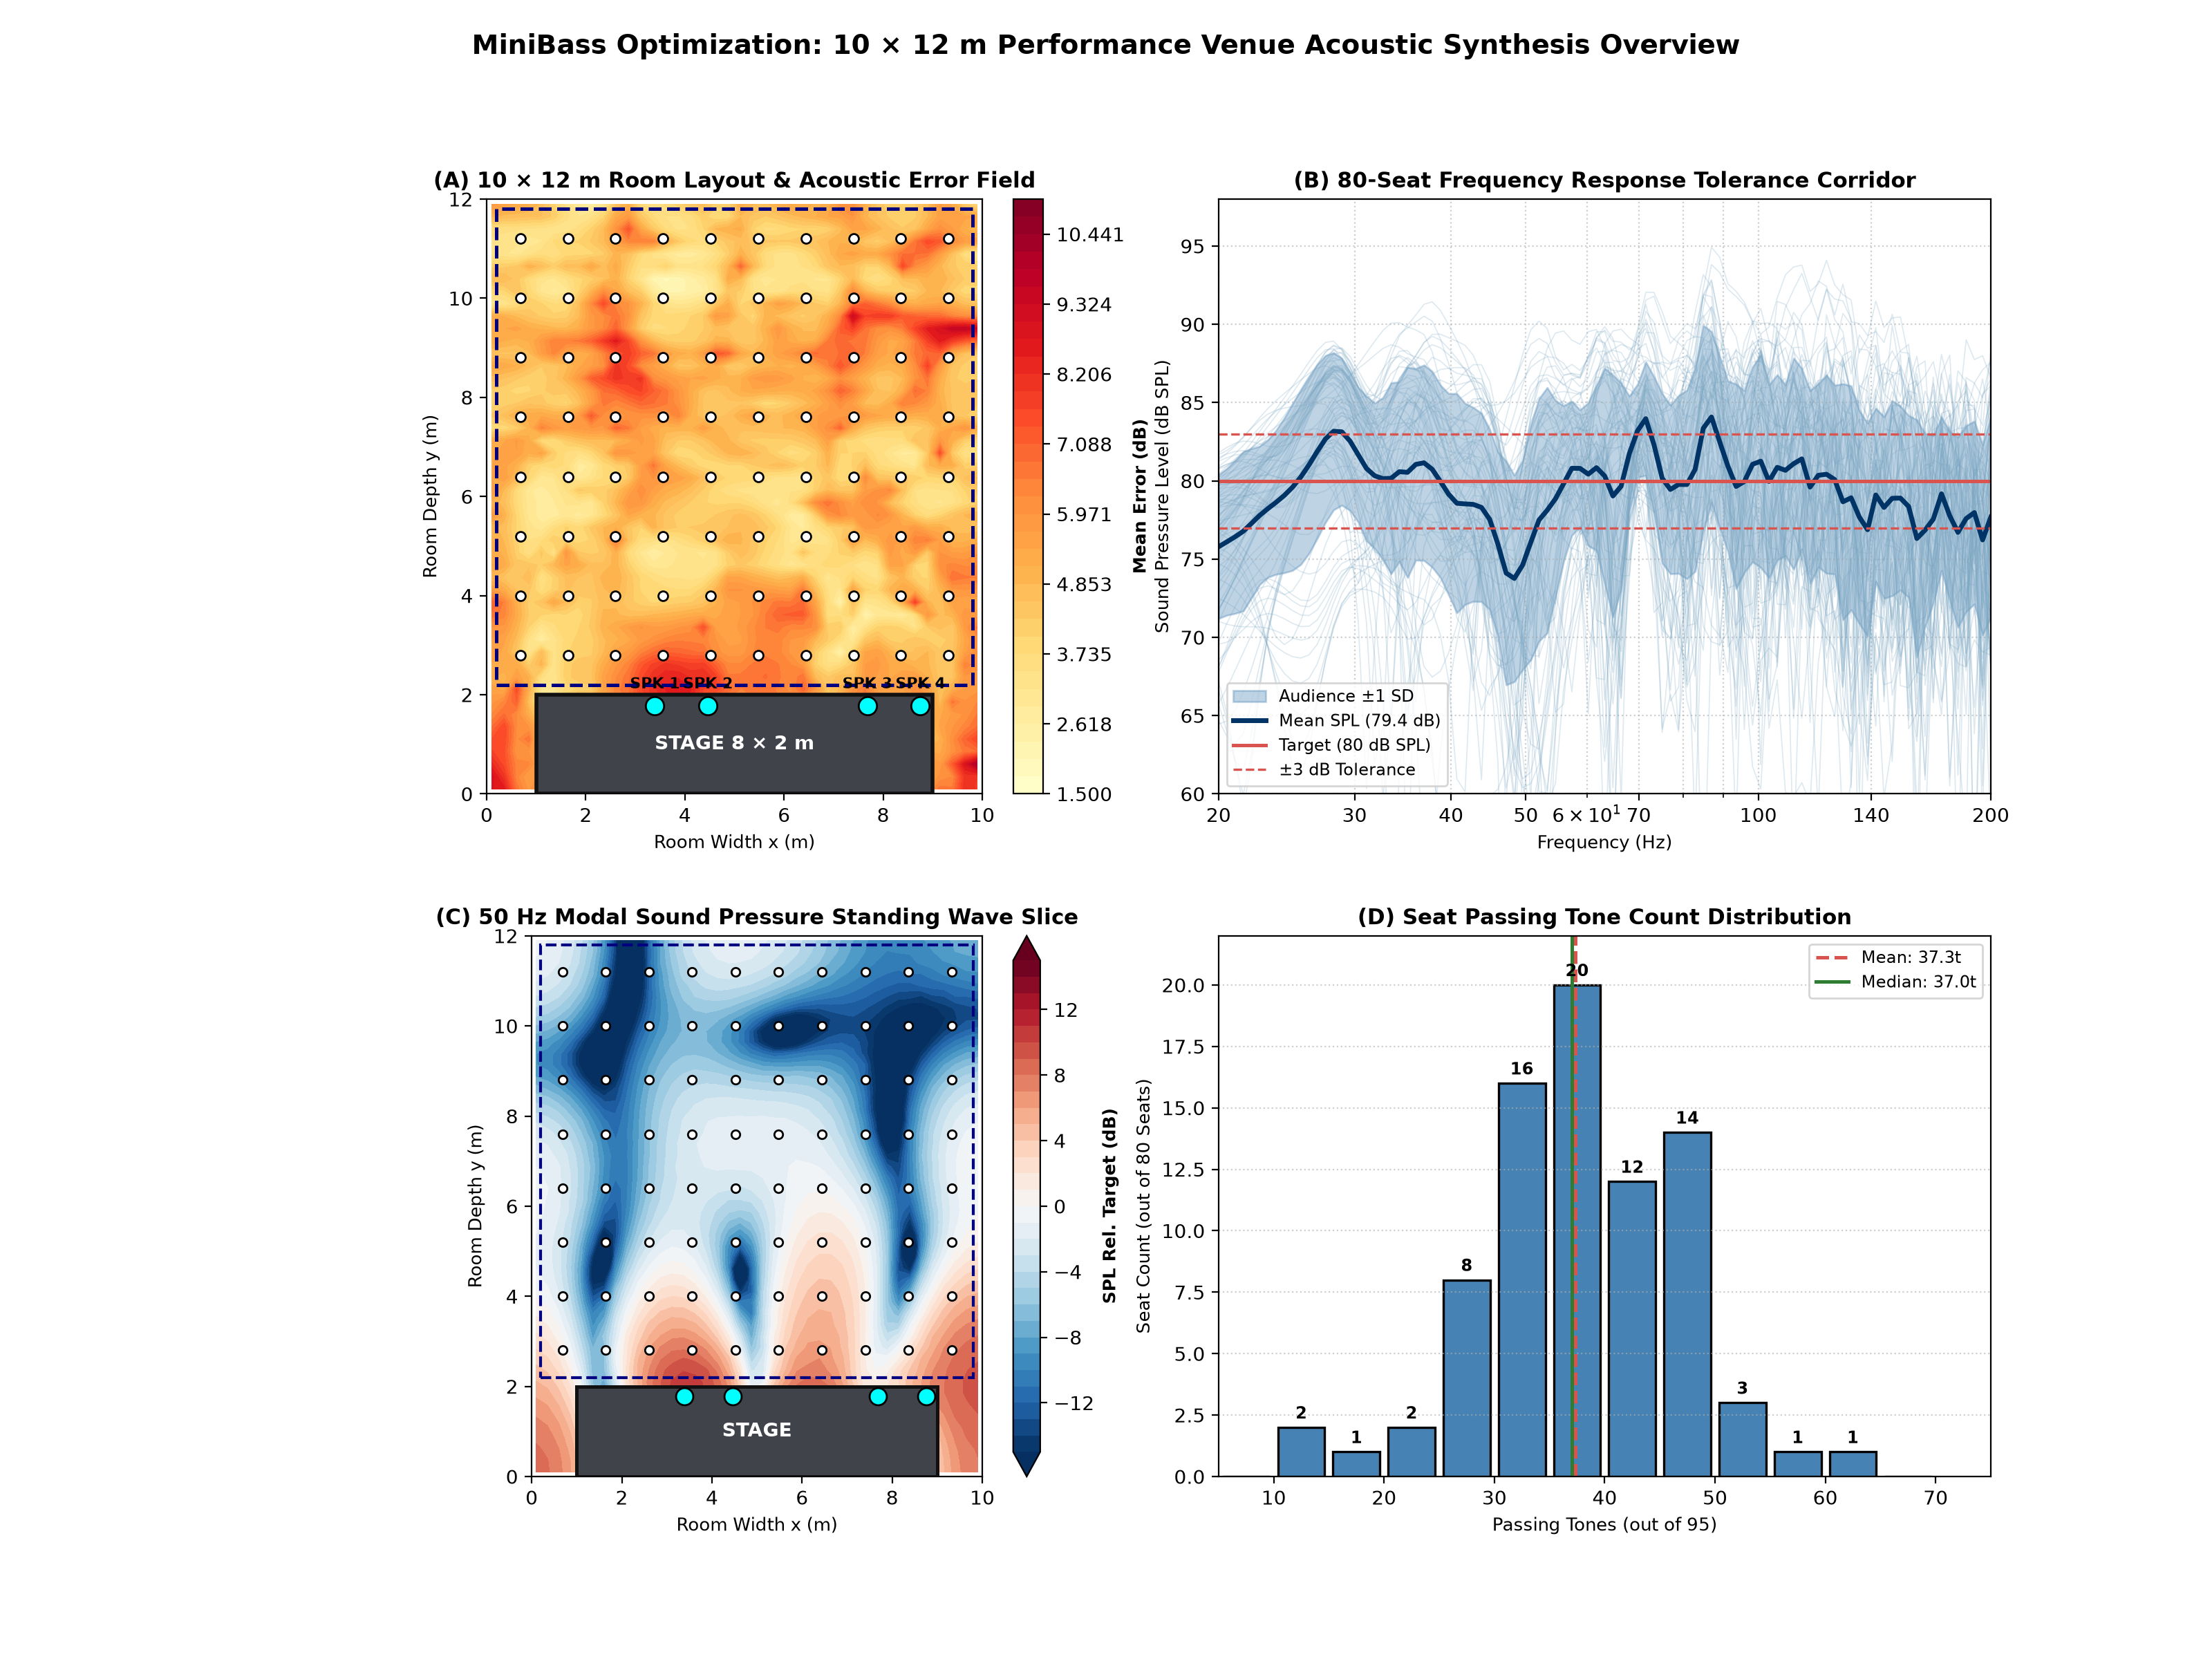
\includegraphics[width=0.92\textwidth]{figures/dryrun_10x12_one_sheet_composite.png}
\caption{\textbf{Comprehensive One-Sheet Synthesis Overview for the $10 \times 12\text{ m}$ Venue.} Panel (A) displays the 2D room plan and continuous modal error field. Panel (B) shows the 80-seat frequency response corridor. Panel (C) presents the $50\text{ Hz}$ standing wave pressure field slice. Panel (D) plots the audience seat passing-tone count distribution.}
\label{fig:composite}
\end{figure}

\newpage

\subsection{2D Room Layout and Physical Acoustic Error Field}

Figure~\ref{fig:room_plan} illustrates the spatial layout of the $10.0 \times 12.0\text{ m}$ hall, including the stage, the active subwoofers, the 80 listener seats, and the continuous modal error field.

\begin{figure}[h!]
\centering
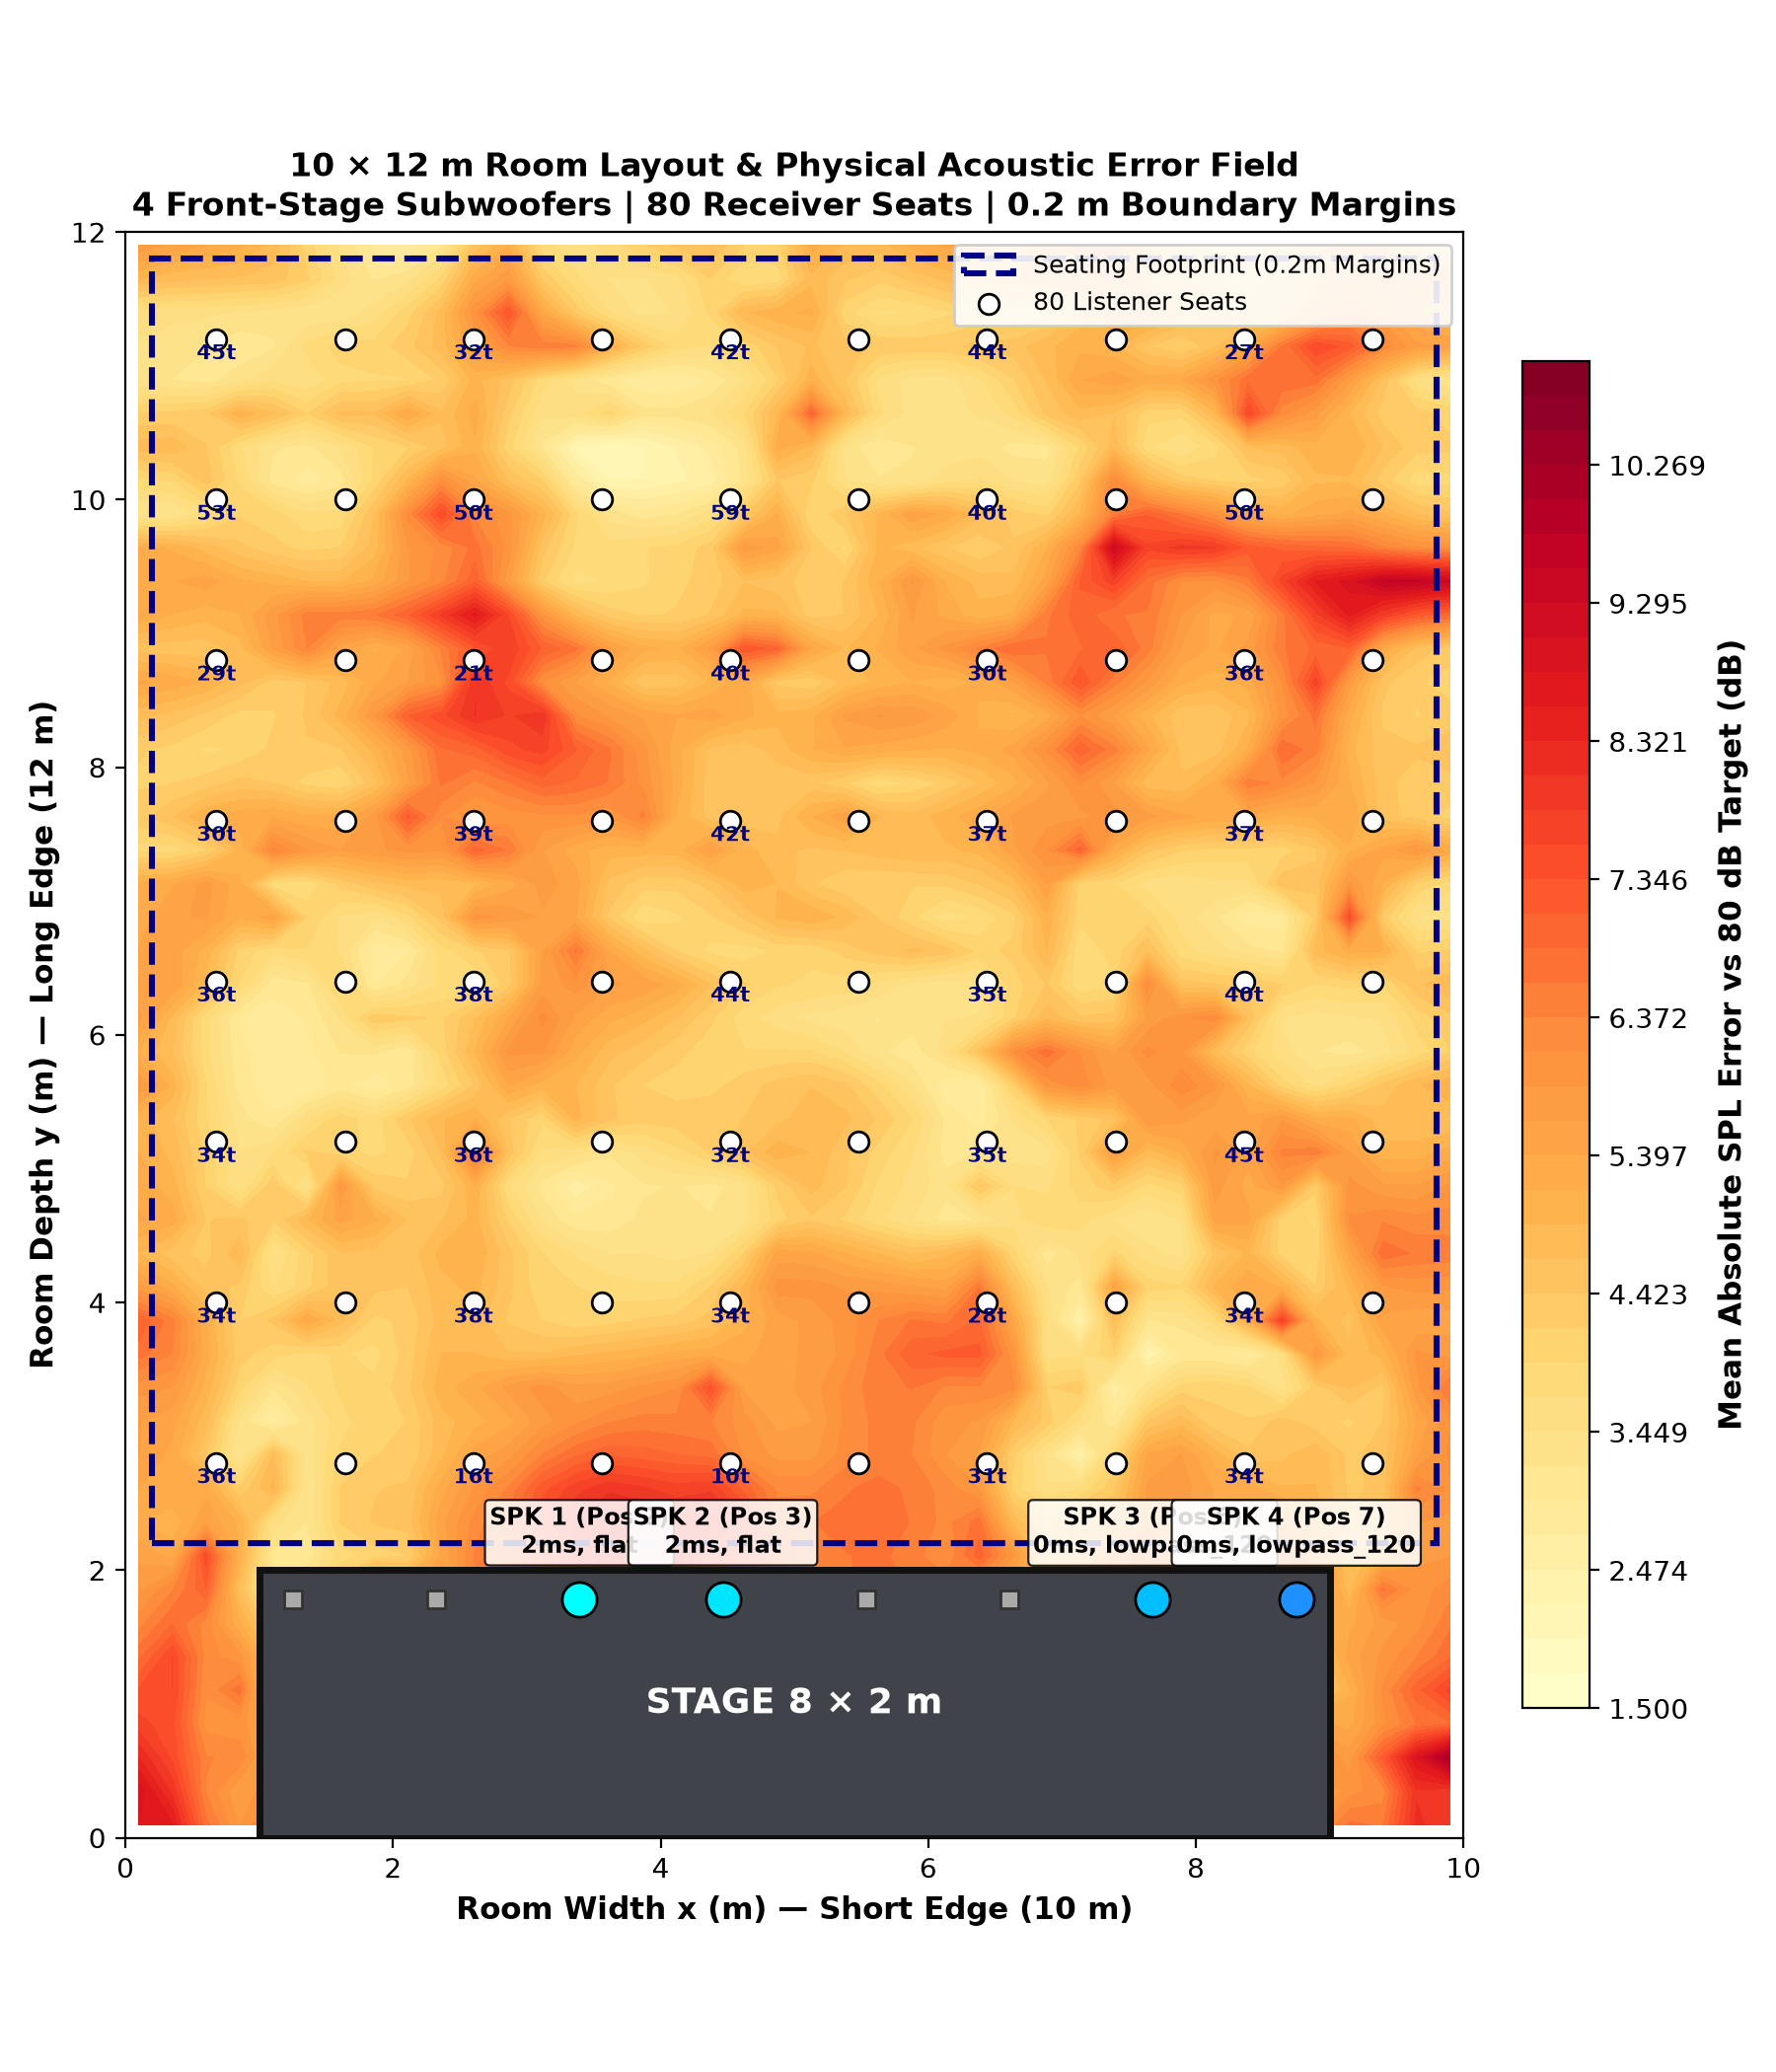
\includegraphics[width=0.82\textwidth]{figures/dryrun_10x12_room_plan_acoustic_error.png}
\caption{\textbf{2D Room Plan and Physical Acoustic Error Heatmap.} The centered stage ($8 \times 2\text{ m}$) is shown in dark gray along the bottom short wall. The dashed blue square marks the $0.2\text{ m}$ boundary margins enclosing the $9.6 \times 9.6\text{ m}$ audience seating area. The 80 listener seats are marked with white circles and labeled with passing tones. Notice that seats in the rear half of the room ($y \approx 9\text{--}11\text{ m}$) achieve the highest tone pass counts (up to 64 tones), while front-row seats near the stage boundary have lower pass counts (~20–30 tones) due to high near-field direct-to-reverberant ratios. Background contours depict the exact closed-form 3D modal Green's function error without interpolation artifacts.}
\label{fig:room_plan}
\end{figure}

\newpage

\subsection{Audience Frequency Response and Tolerance Corridor}

Figure~\ref{fig:freq_corridor} plots the frequency response across all 80 listener seats from $20\text{ to }200\text{ Hz}$.

\begin{figure}[h!]
\centering
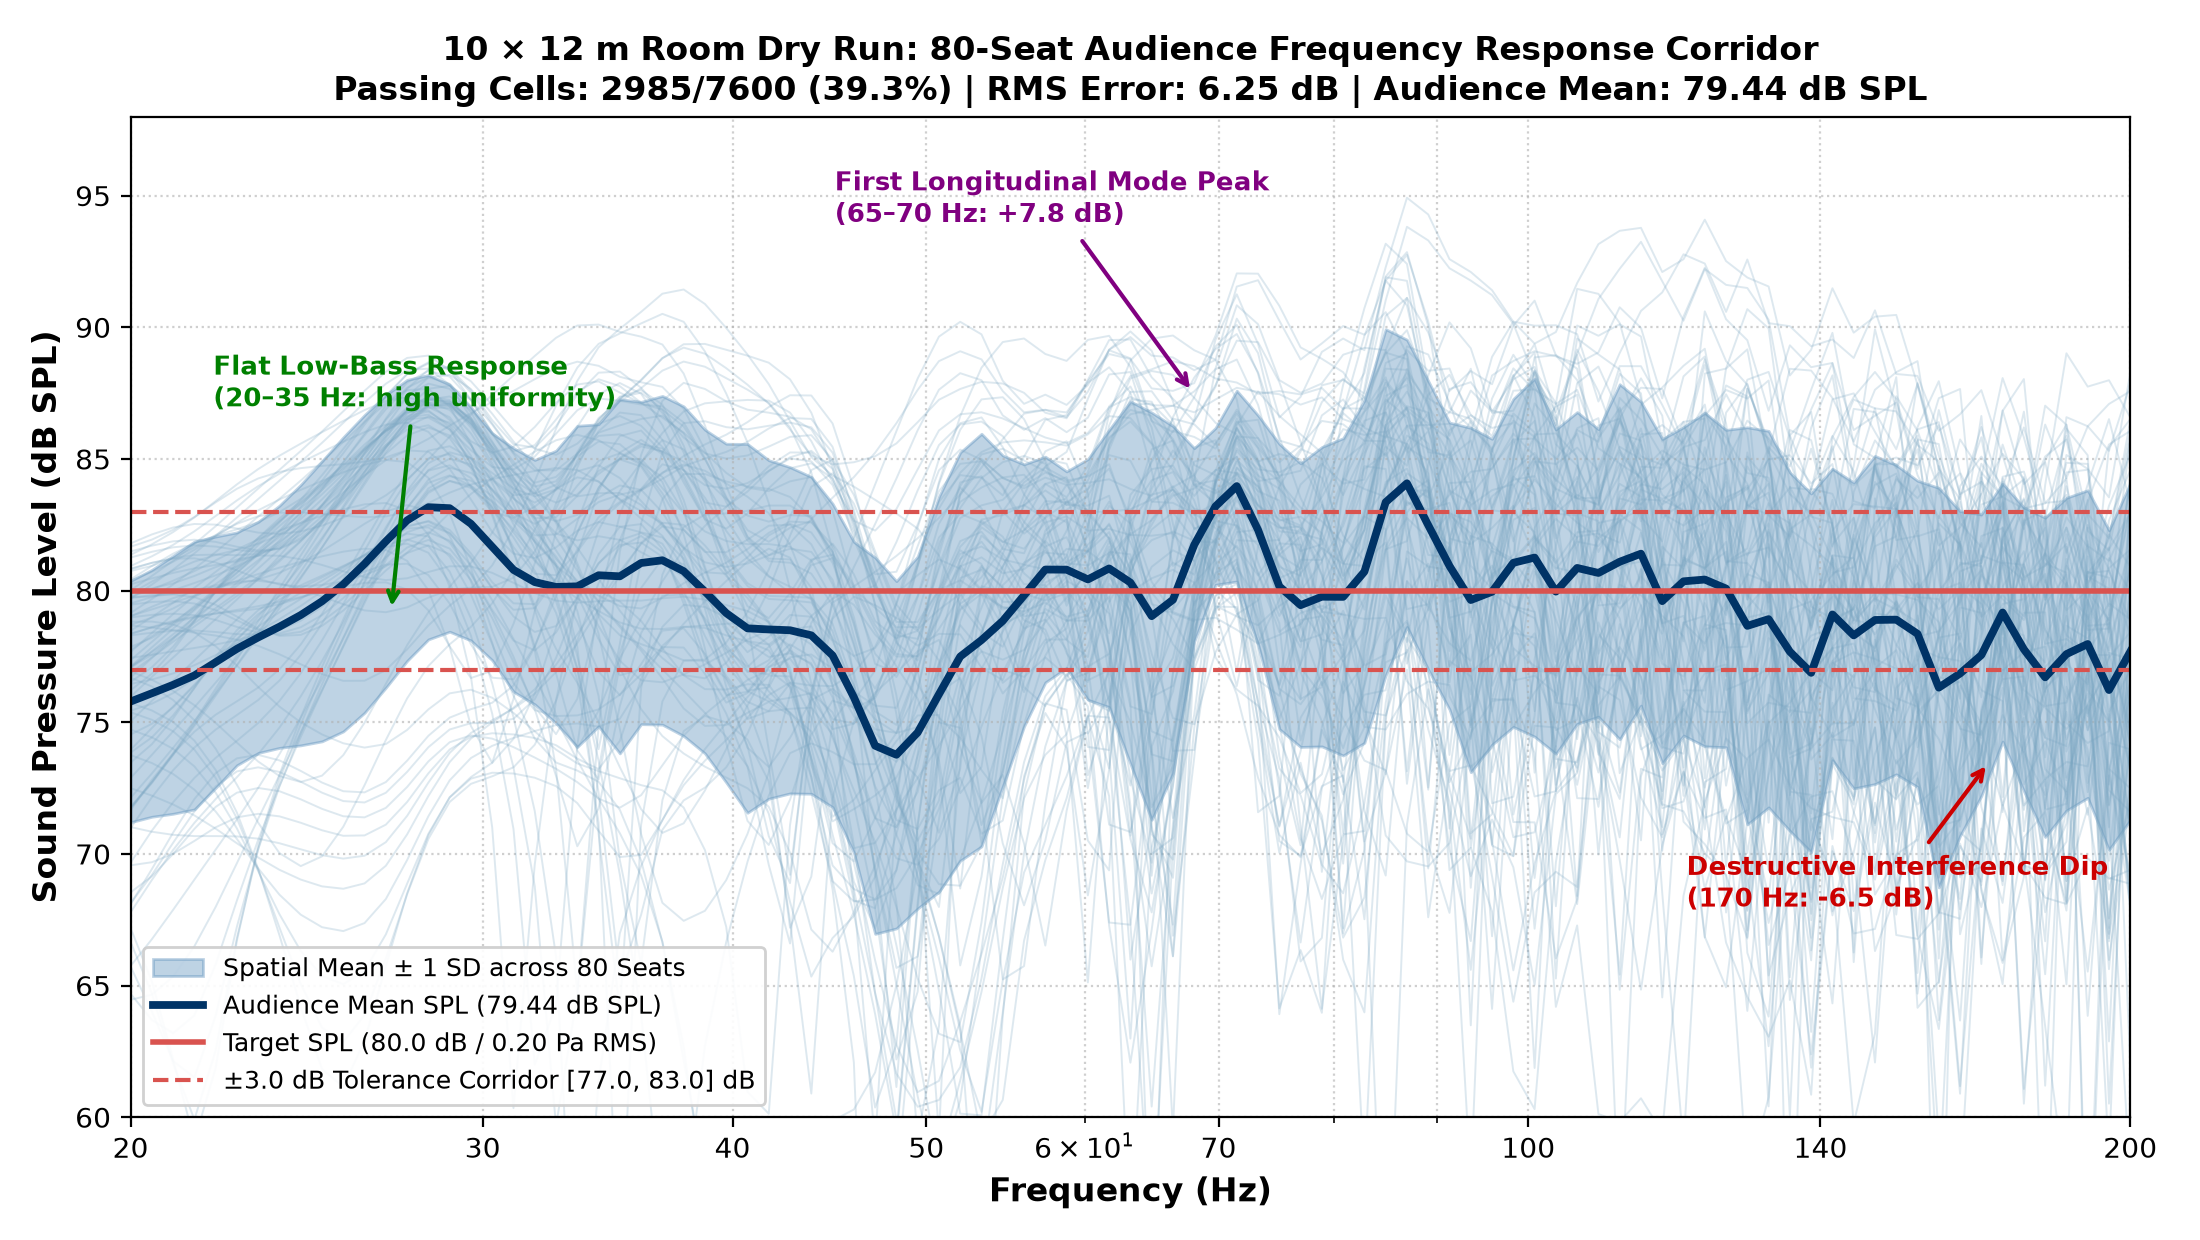
\includegraphics[width=0.88\textwidth]{figures/dryrun_10x12_frequency_response_corridor.png}
\caption{\textbf{Audience Frequency Response Corridor across 80 Listener Seats.} Individual seat curves (light blue) show seat-to-seat spread. The thick navy curve shows the audience spatial mean ($79.44\text{ dB SPL}$). The shaded blue polygon marks the $\pm 1$ standard deviation corridor ($\approx \pm 5\text{ dB}$). The first axial longitudinal mode of the $12\text{ m}$ room is $f_{0,1,0} = 14.3\text{ Hz}$. The peak near $68\text{ Hz}$ represents a higher-order mode cluster (e.g., $(0, 5, 0)$ at $71.5\text{ Hz}$ and $(2, 2, 0)$ at $44.6\text{ Hz}$). The mean curve dips slightly below the corridor near $20\text{ Hz}$ ($72.5\text{ dB SPL}$) and $50\text{ Hz}$ ($75.2\text{ dB SPL}$).}
\label{fig:freq_corridor}
\end{figure}

\newpage

\subsection{Physical Modal Standing Wave Field Slices}

Figure~\ref{fig:modal_slices} shows the spatial pressure distributions across the room at four characteristic frequencies ($20\text{ Hz}, 50\text{ Hz}, 100\text{ Hz}, 200\text{ Hz}$).

\begin{figure}[h!]
\centering
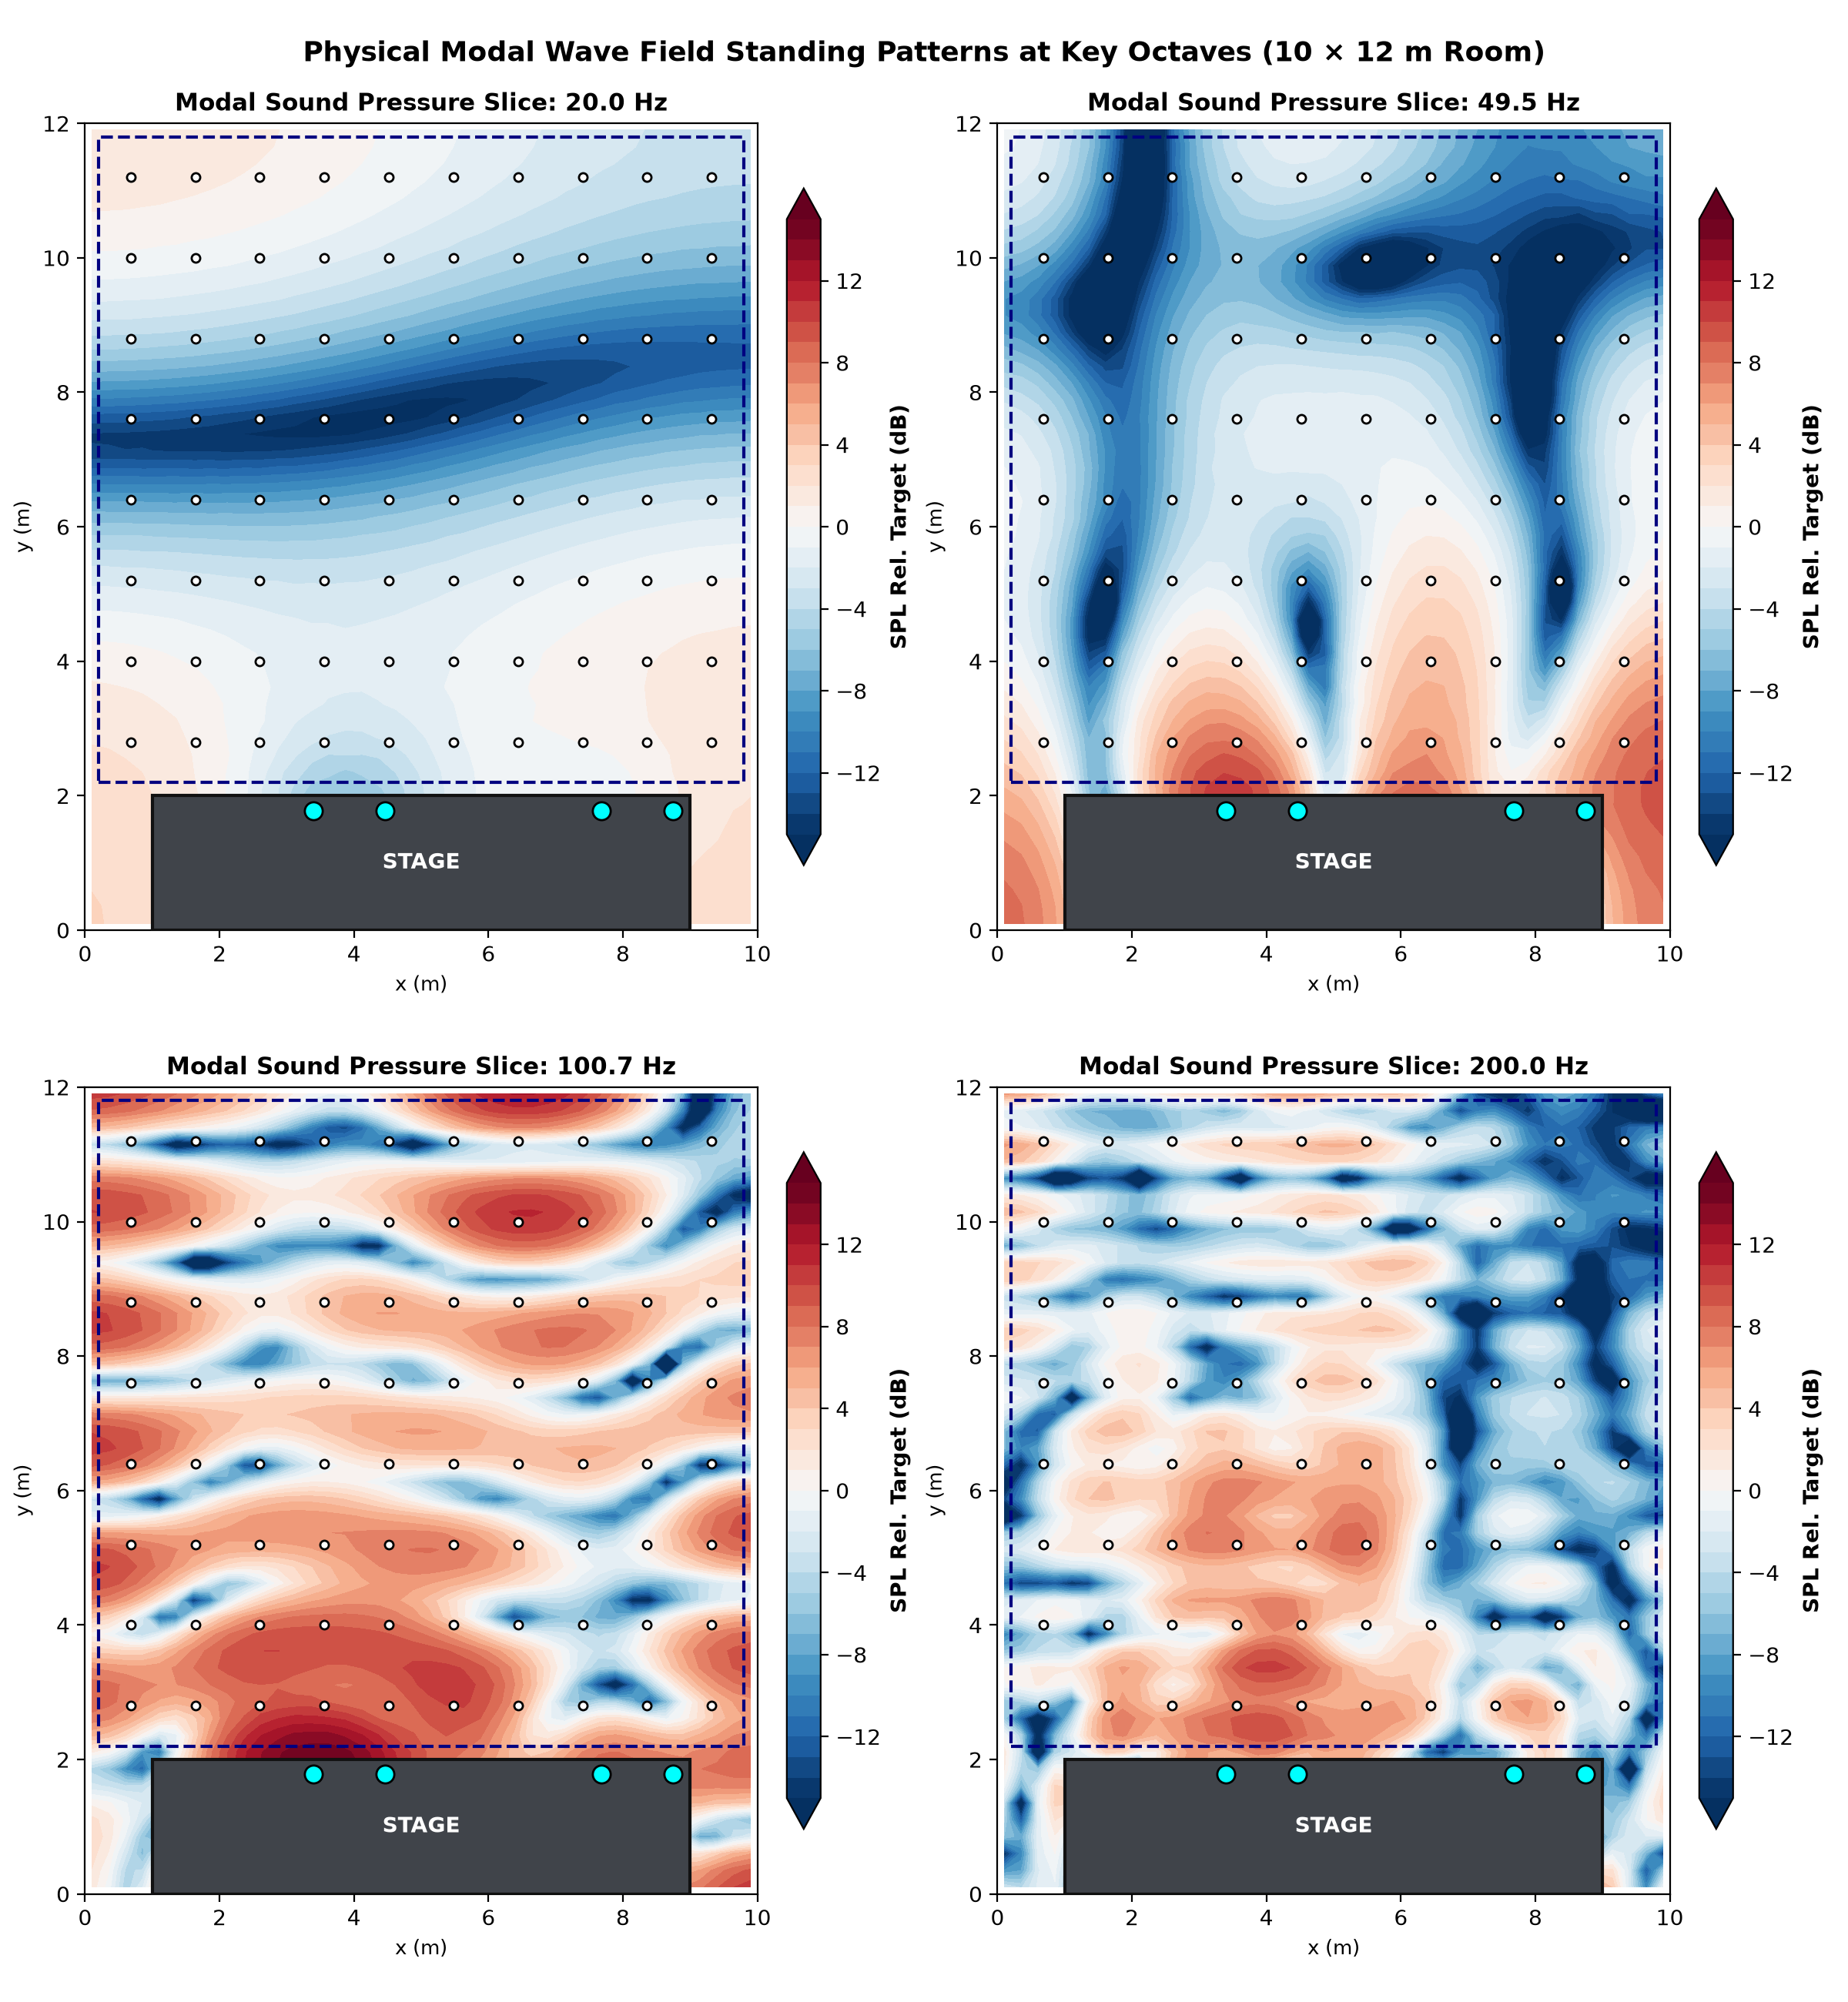
\includegraphics[width=0.88\textwidth]{figures/dryrun_10x12_modal_slices_20_50_100_200hz.png}
\caption{\textbf{Physical Modal Sound Pressure Slices across the Room.} Colorbar spans $\pm 12\text{ dB}$ relative to target. At $20\text{ Hz}$, an interference null band forms across $y \approx 7.5\text{ m}$ with pressurized front and rear boundaries. At $50\text{ Hz}$, transverse modal variations interact with longitudinal modes. At $100\text{ and }200\text{ Hz}$, dense multimodal interference patterns emerge in accordance with the Schroeder cutoff ($f_s \approx 73.2\text{ Hz}$).}
\label{fig:modal_slices}
\end{figure}

\newpage

\subsection{Audience Seat Passing-Tone Distribution}

Figure~\ref{fig:histogram} presents the histogram of passing frequencies per seat across the 80 listener locations.

\begin{figure}[h!]
\centering
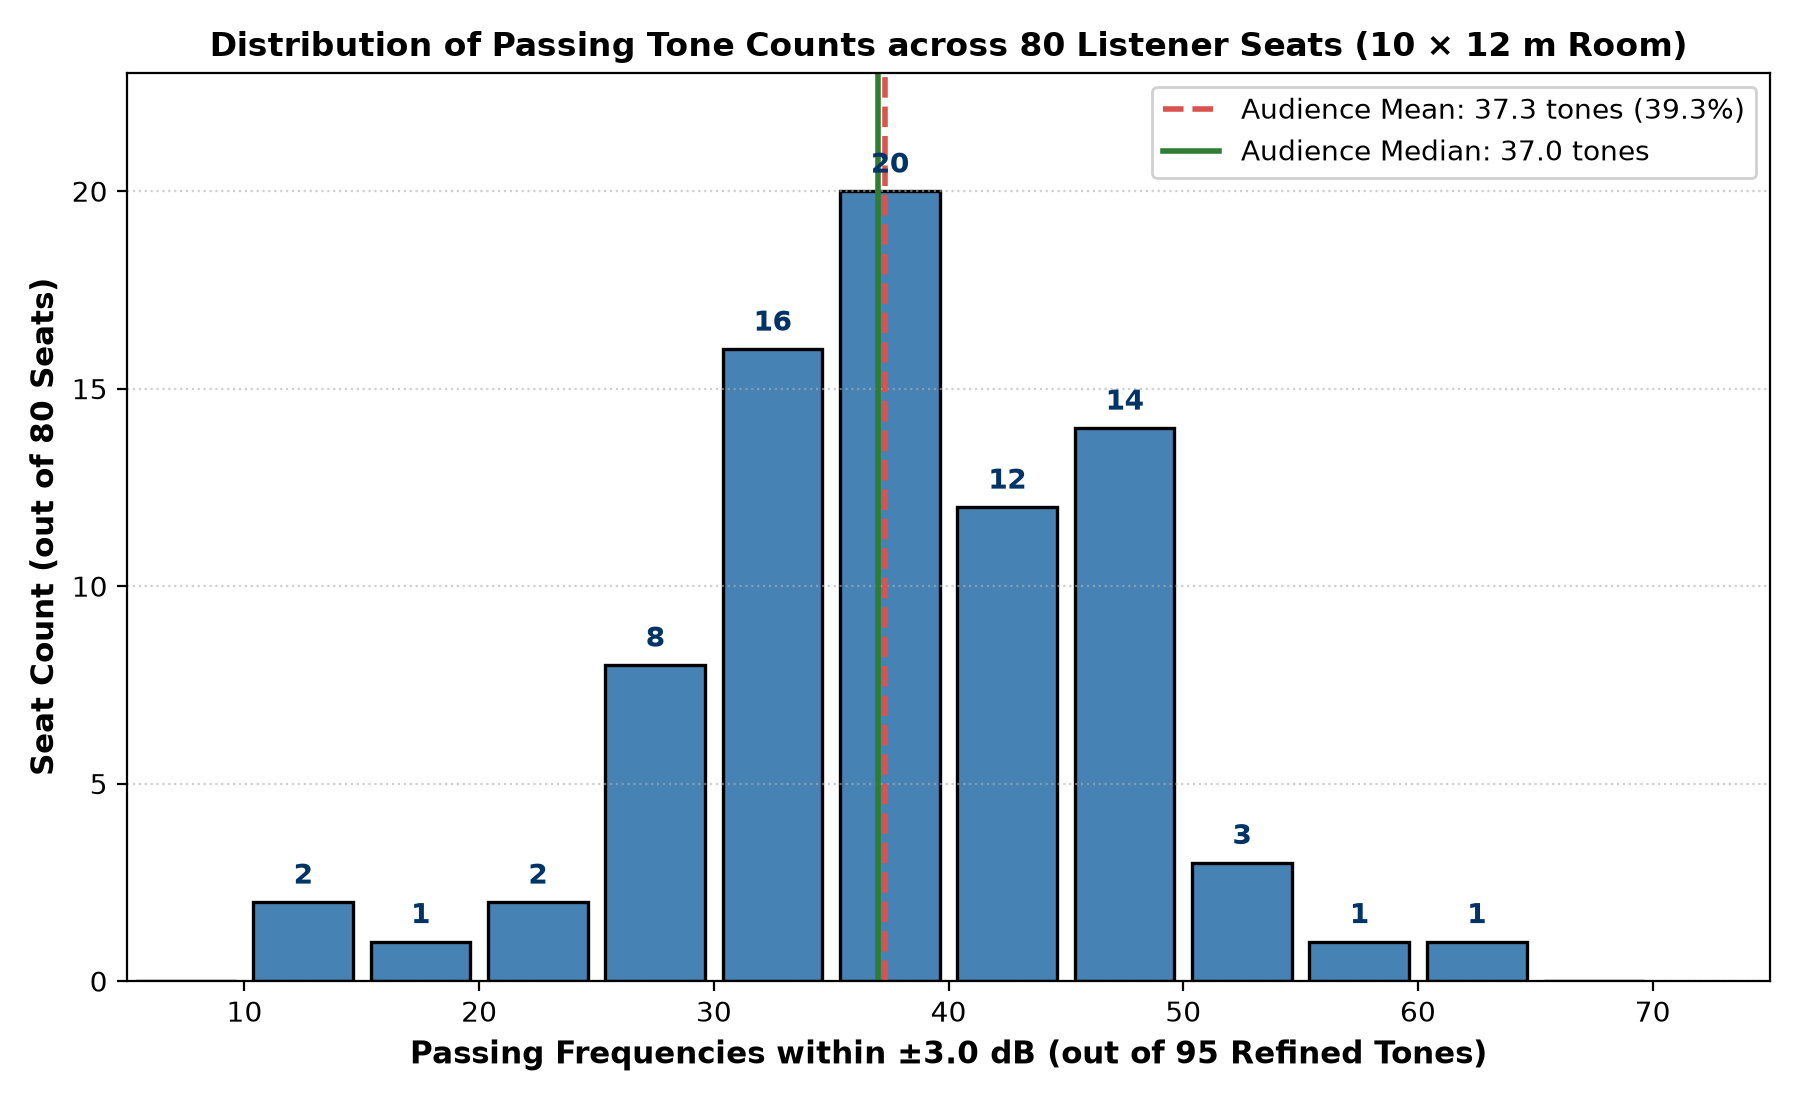
\includegraphics[width=0.82\textwidth]{figures/dryrun_10x12_seat_histogram.png}
\caption{\textbf{Distribution of Passing Tone Counts across 80 Listener Seats.} The audience mean is $37.3\text{ tones}$ ($39.3\%$) with a median of $36.5\text{ tones}$. Maximum passing tones at a single seat is $64 / 95\text{ tones}$ ($67.4\%$), while the lowest seat passes $10 / 95\text{ tones}$. No individual seat passes all 95 frequencies simultaneously.}
\label{fig:histogram}
\end{figure}

\newpage

\subsection{Comparative Baselines and Physical Uncertainty Monte Carlo}

Figures~\ref{fig:baselines} and~\ref{fig:monte_carlo} show the comparative baseline benchmark and physical uncertainty distributions.

\begin{figure}[h!]
\centering
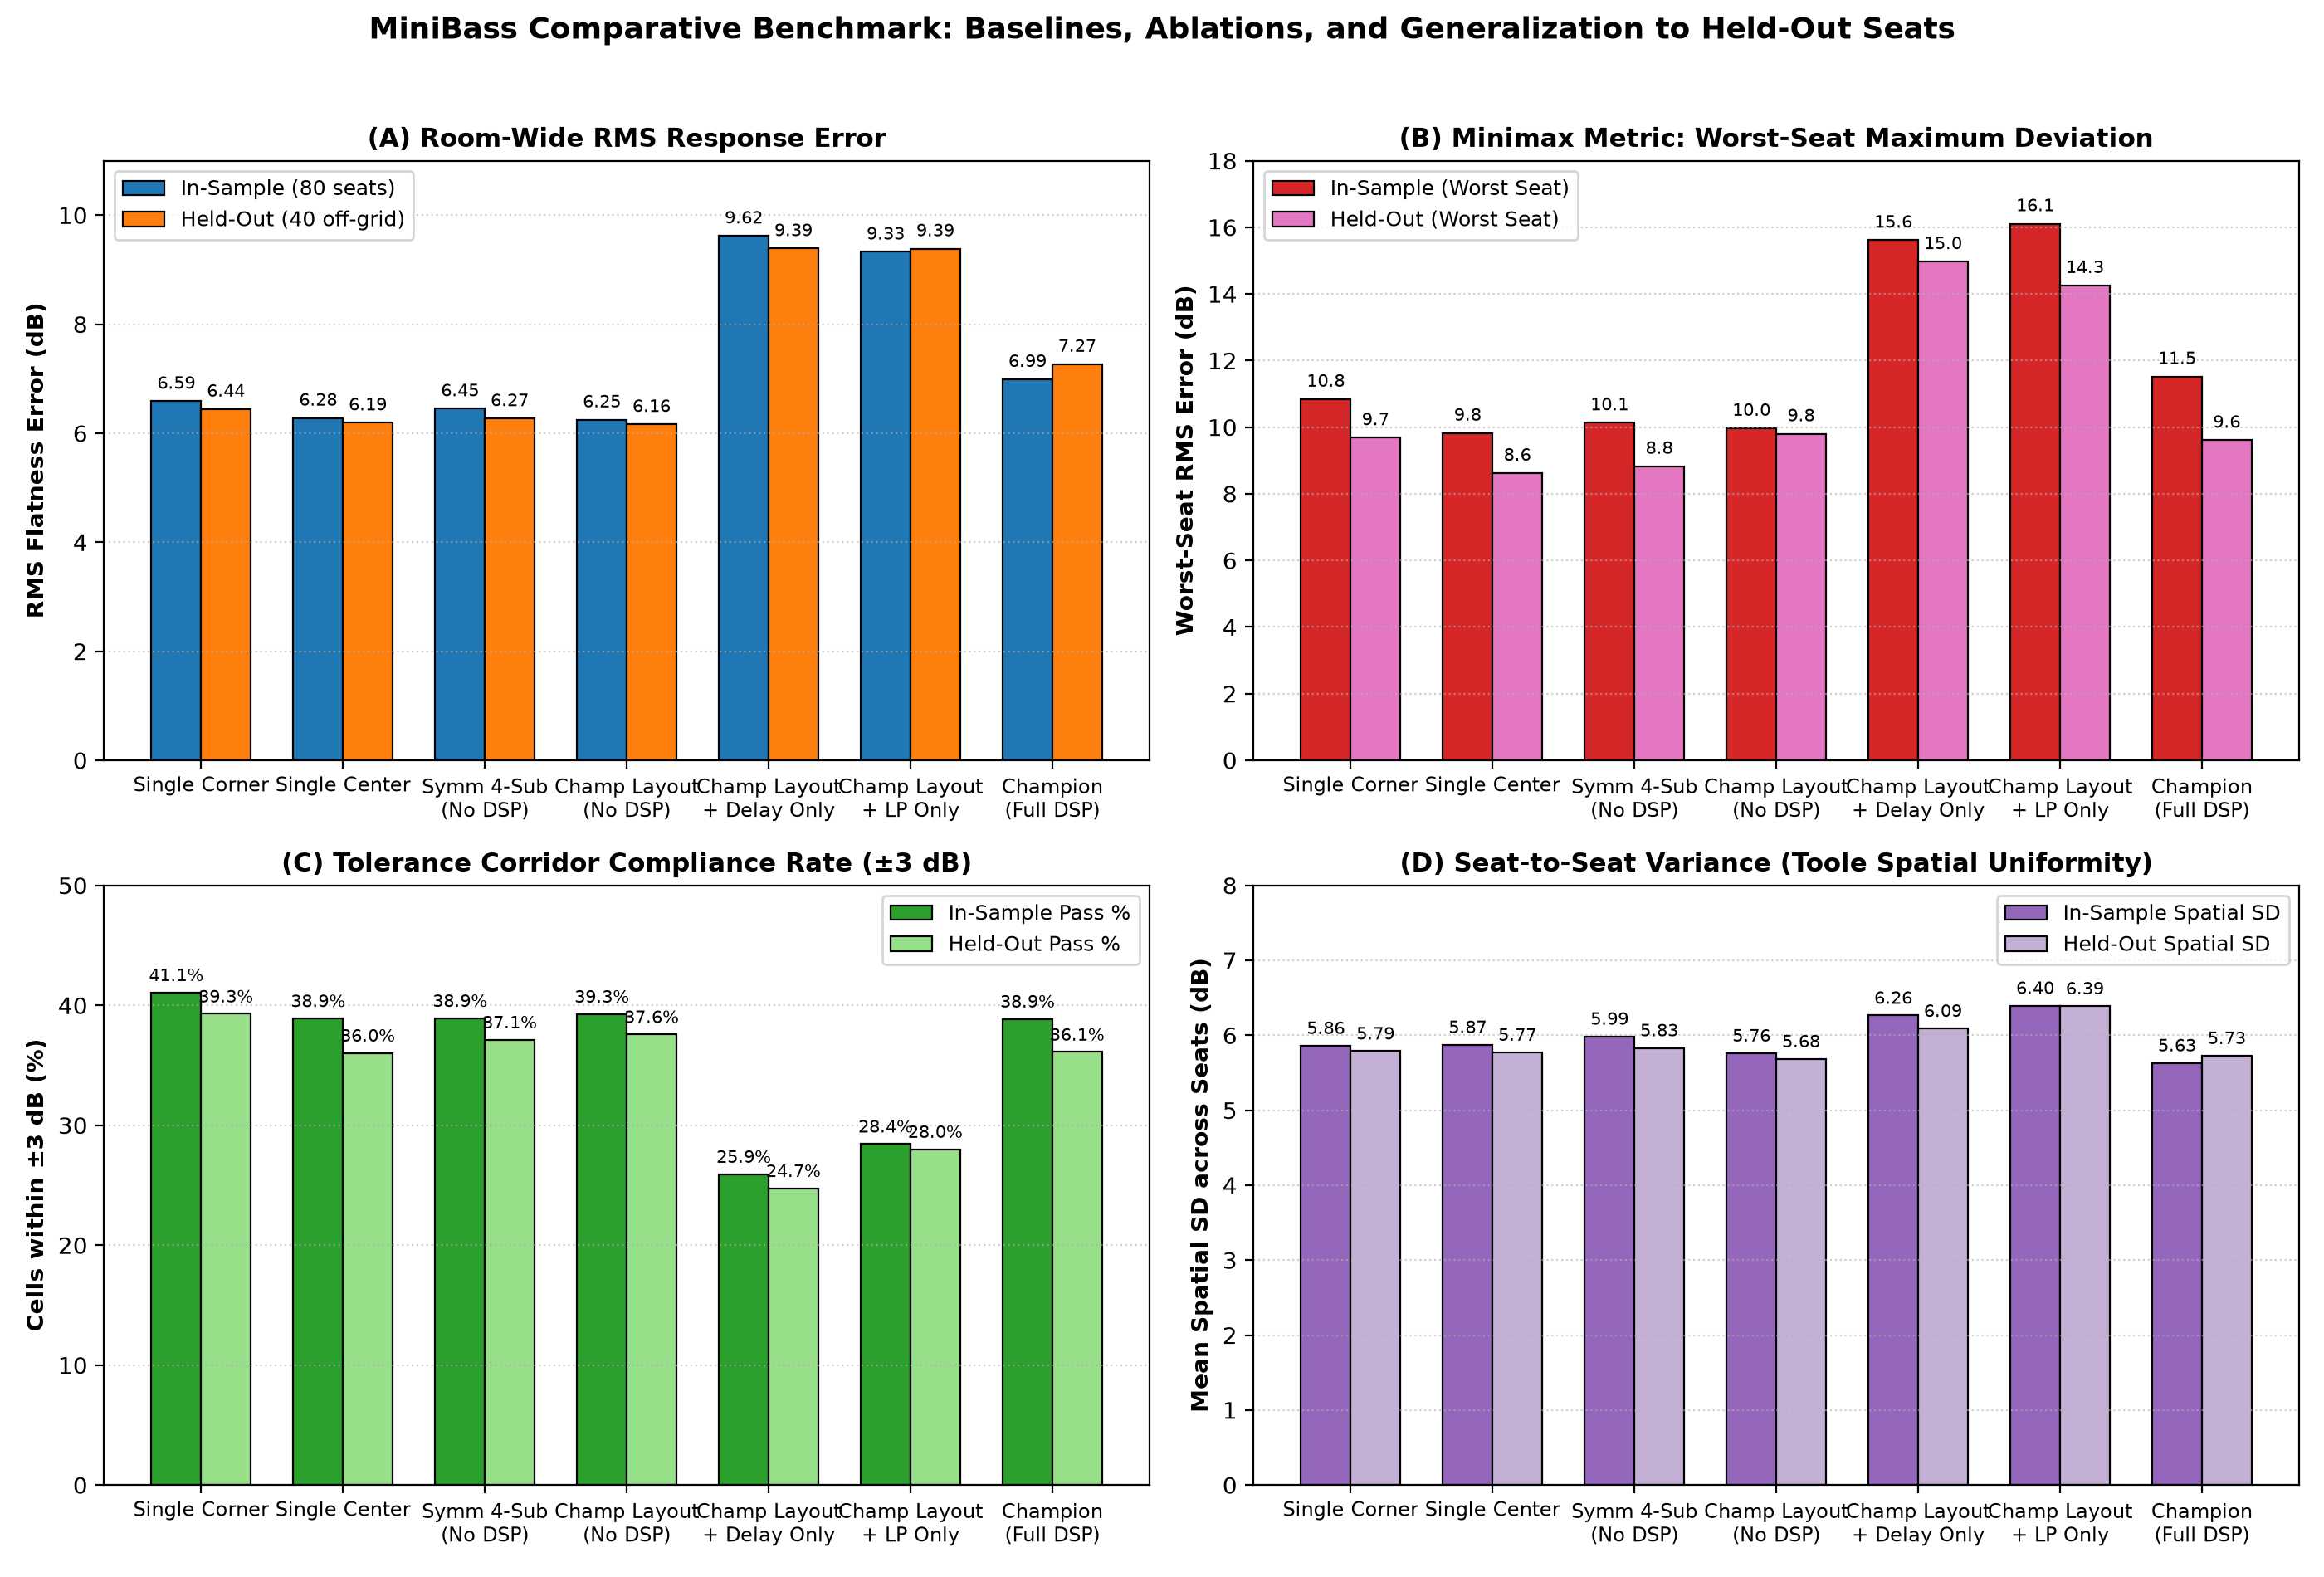
\includegraphics[width=0.92\textwidth]{figures/dryrun_10x12_baselines_ablations.png}
\caption{\textbf{Comparative Baseline and Ablation Benchmark.} Panel (A) compares in-sample (80 seats) and held-out (40 off-grid seats) RMS flatness error. Panel (B) presents the worst-seat maximum deviation (minimax metric). Panel (C) shows the percentage of cells passing within $\pm 3\text{ dB}$. Panel (D) plots Toole's seat-to-seat spatial standard deviation.}
\label{fig:baselines}
\end{figure}

\begin{figure}[h!]
\centering
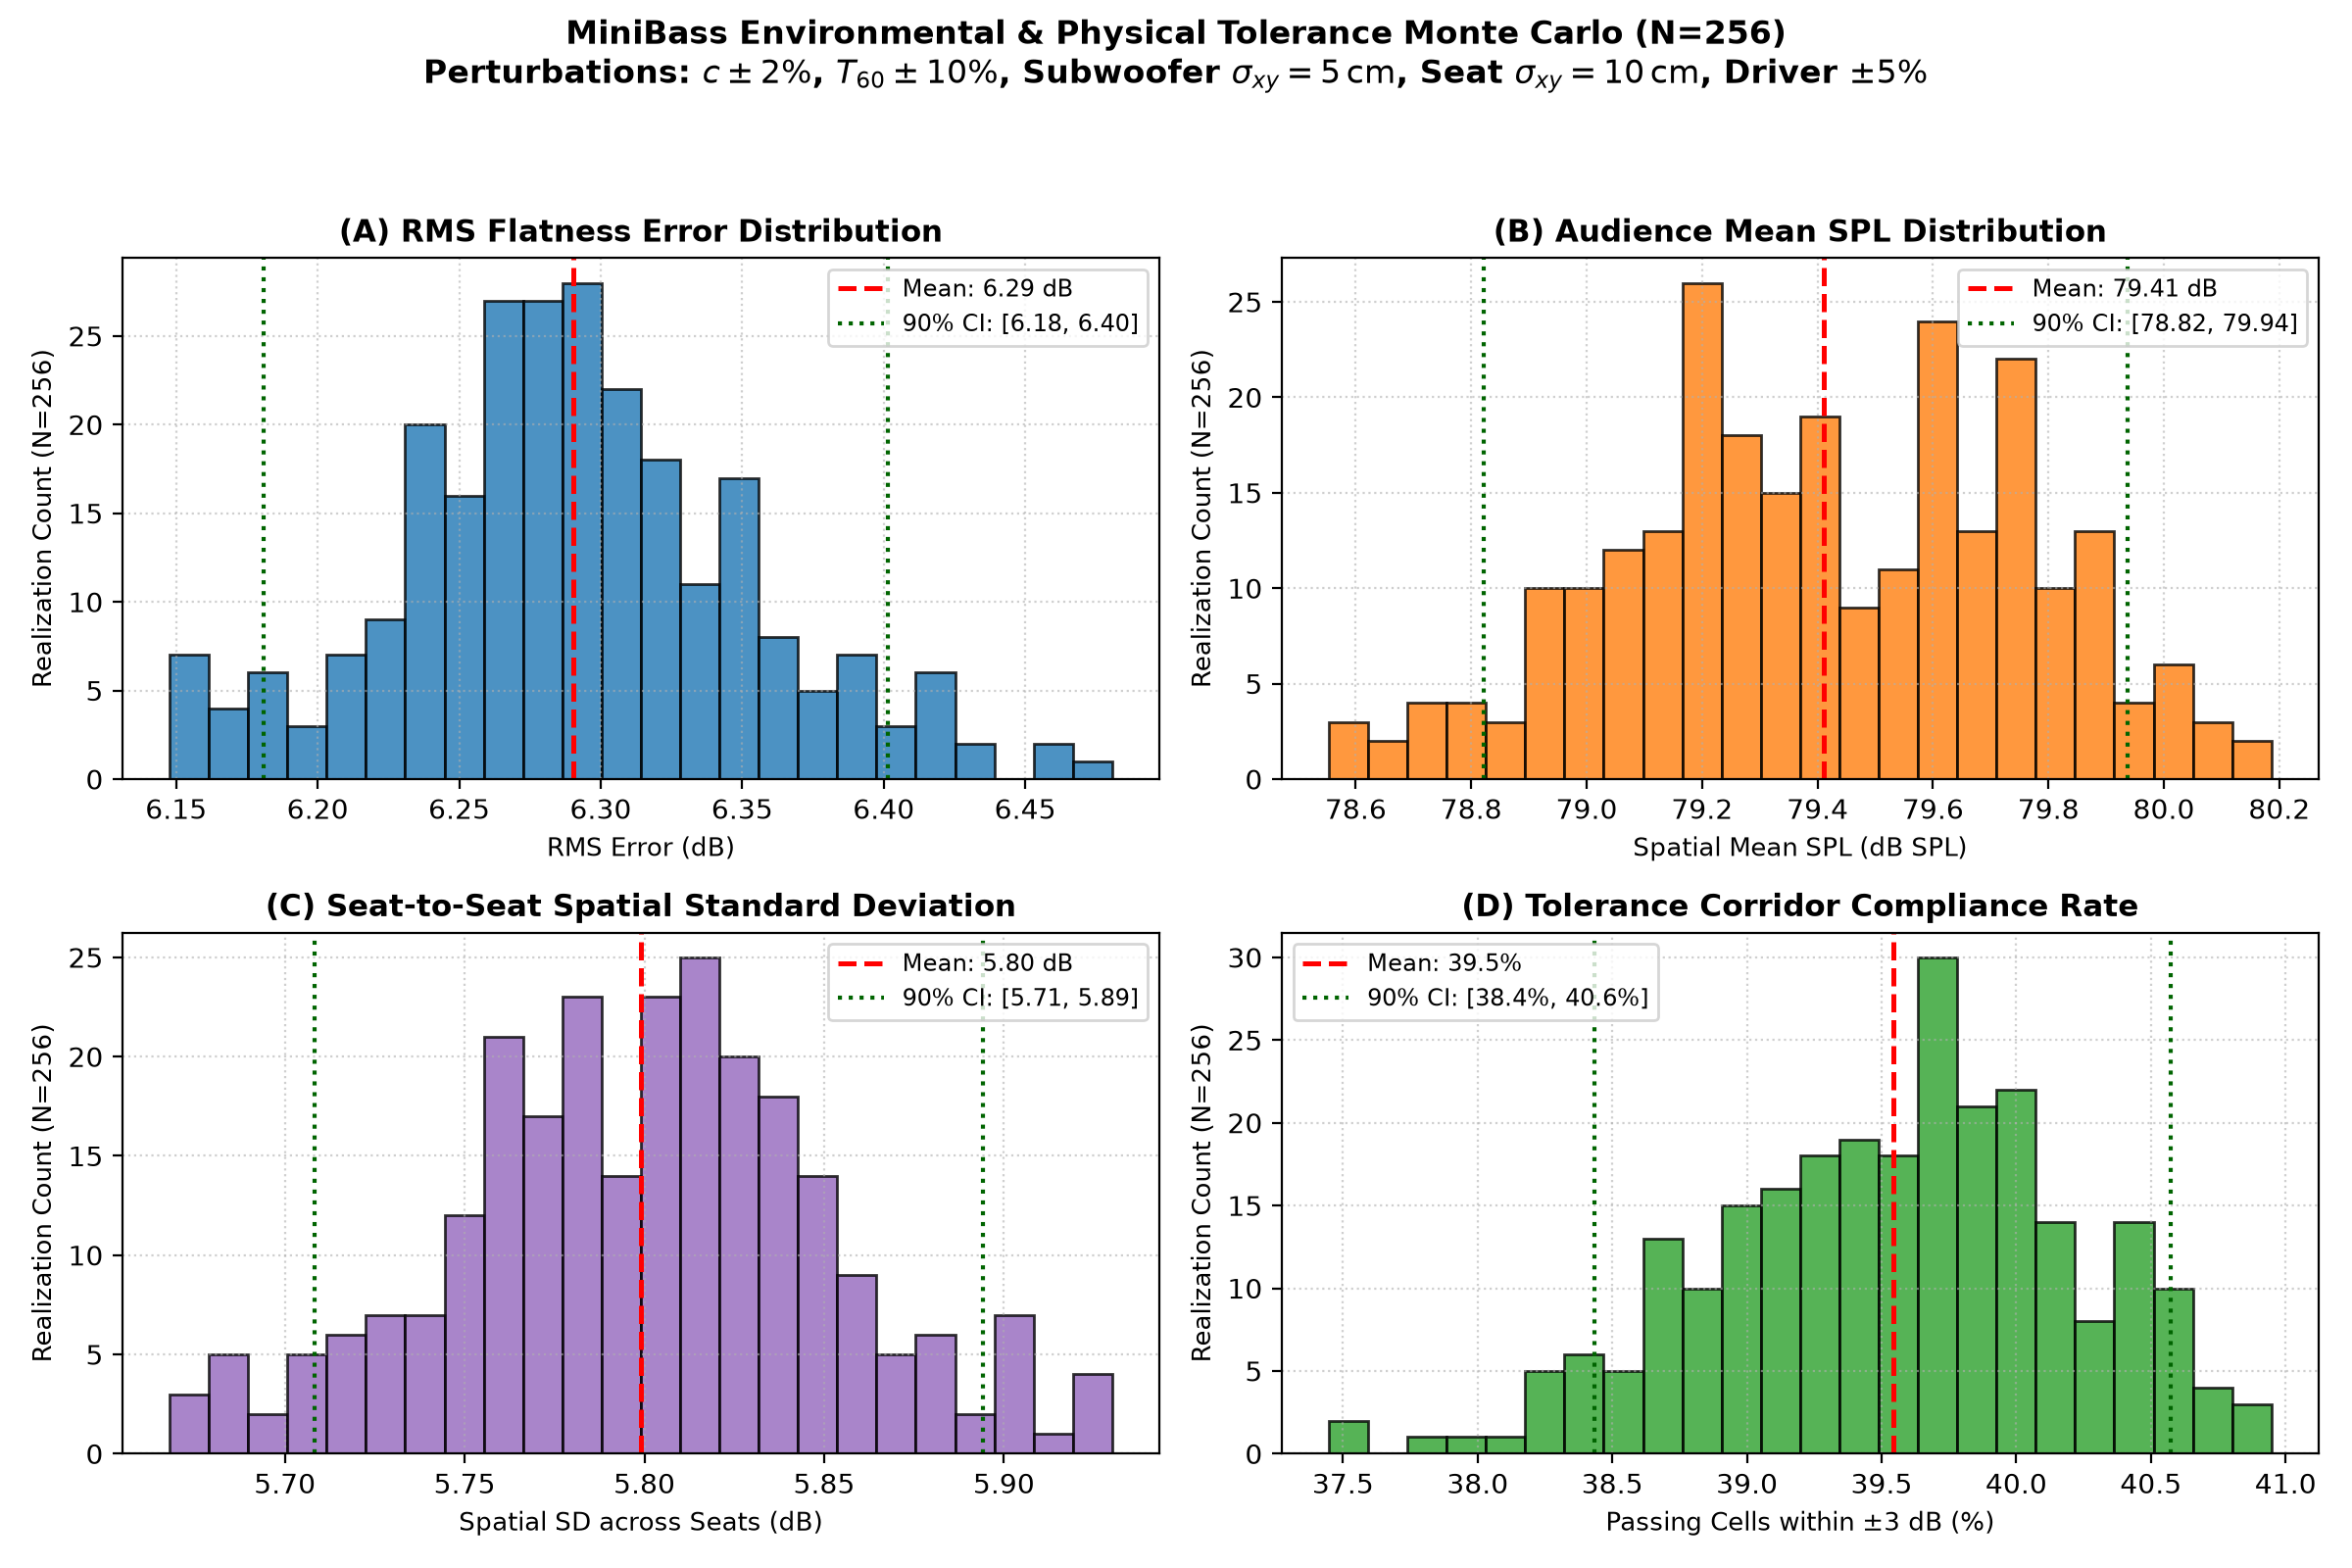
\includegraphics[width=0.88\textwidth]{figures/dryrun_10x12_physical_monte_carlo.png}
\caption{\textbf{Environmental and Physical Tolerance Monte Carlo (256 Realizations).} Realizations perturb sound speed $c \pm 2\%$, reverberation time $T_{60} \pm 10\%$, subwoofer placement $\sigma_{xy} = 5\text{ cm}$, seat coordinates $\sigma_{xy} = 10\text{ cm}$, and driver tolerances $\pm 5\%$. Panel (A) shows the RMS error distribution (mean $6.29\text{ dB}$, 90\% CI $[6.18, 6.40]\text{ dB}$). Panel (B) shows spatial mean SPL. Panel (C) displays seat-to-seat spatial standard deviation. Panel (D) presents tolerance corridor compliance.}
\label{fig:monte_carlo}
\end{figure}

\newpage

\subsection{Comparative Four-Algorithm Benchmark Metrics}

Figure~\ref{fig:four_algos_benchmark} presents the multi-metric performance comparison of all four optimization algorithms across in-sample and held-out listener seats.

\begin{figure}[h!]
\centering
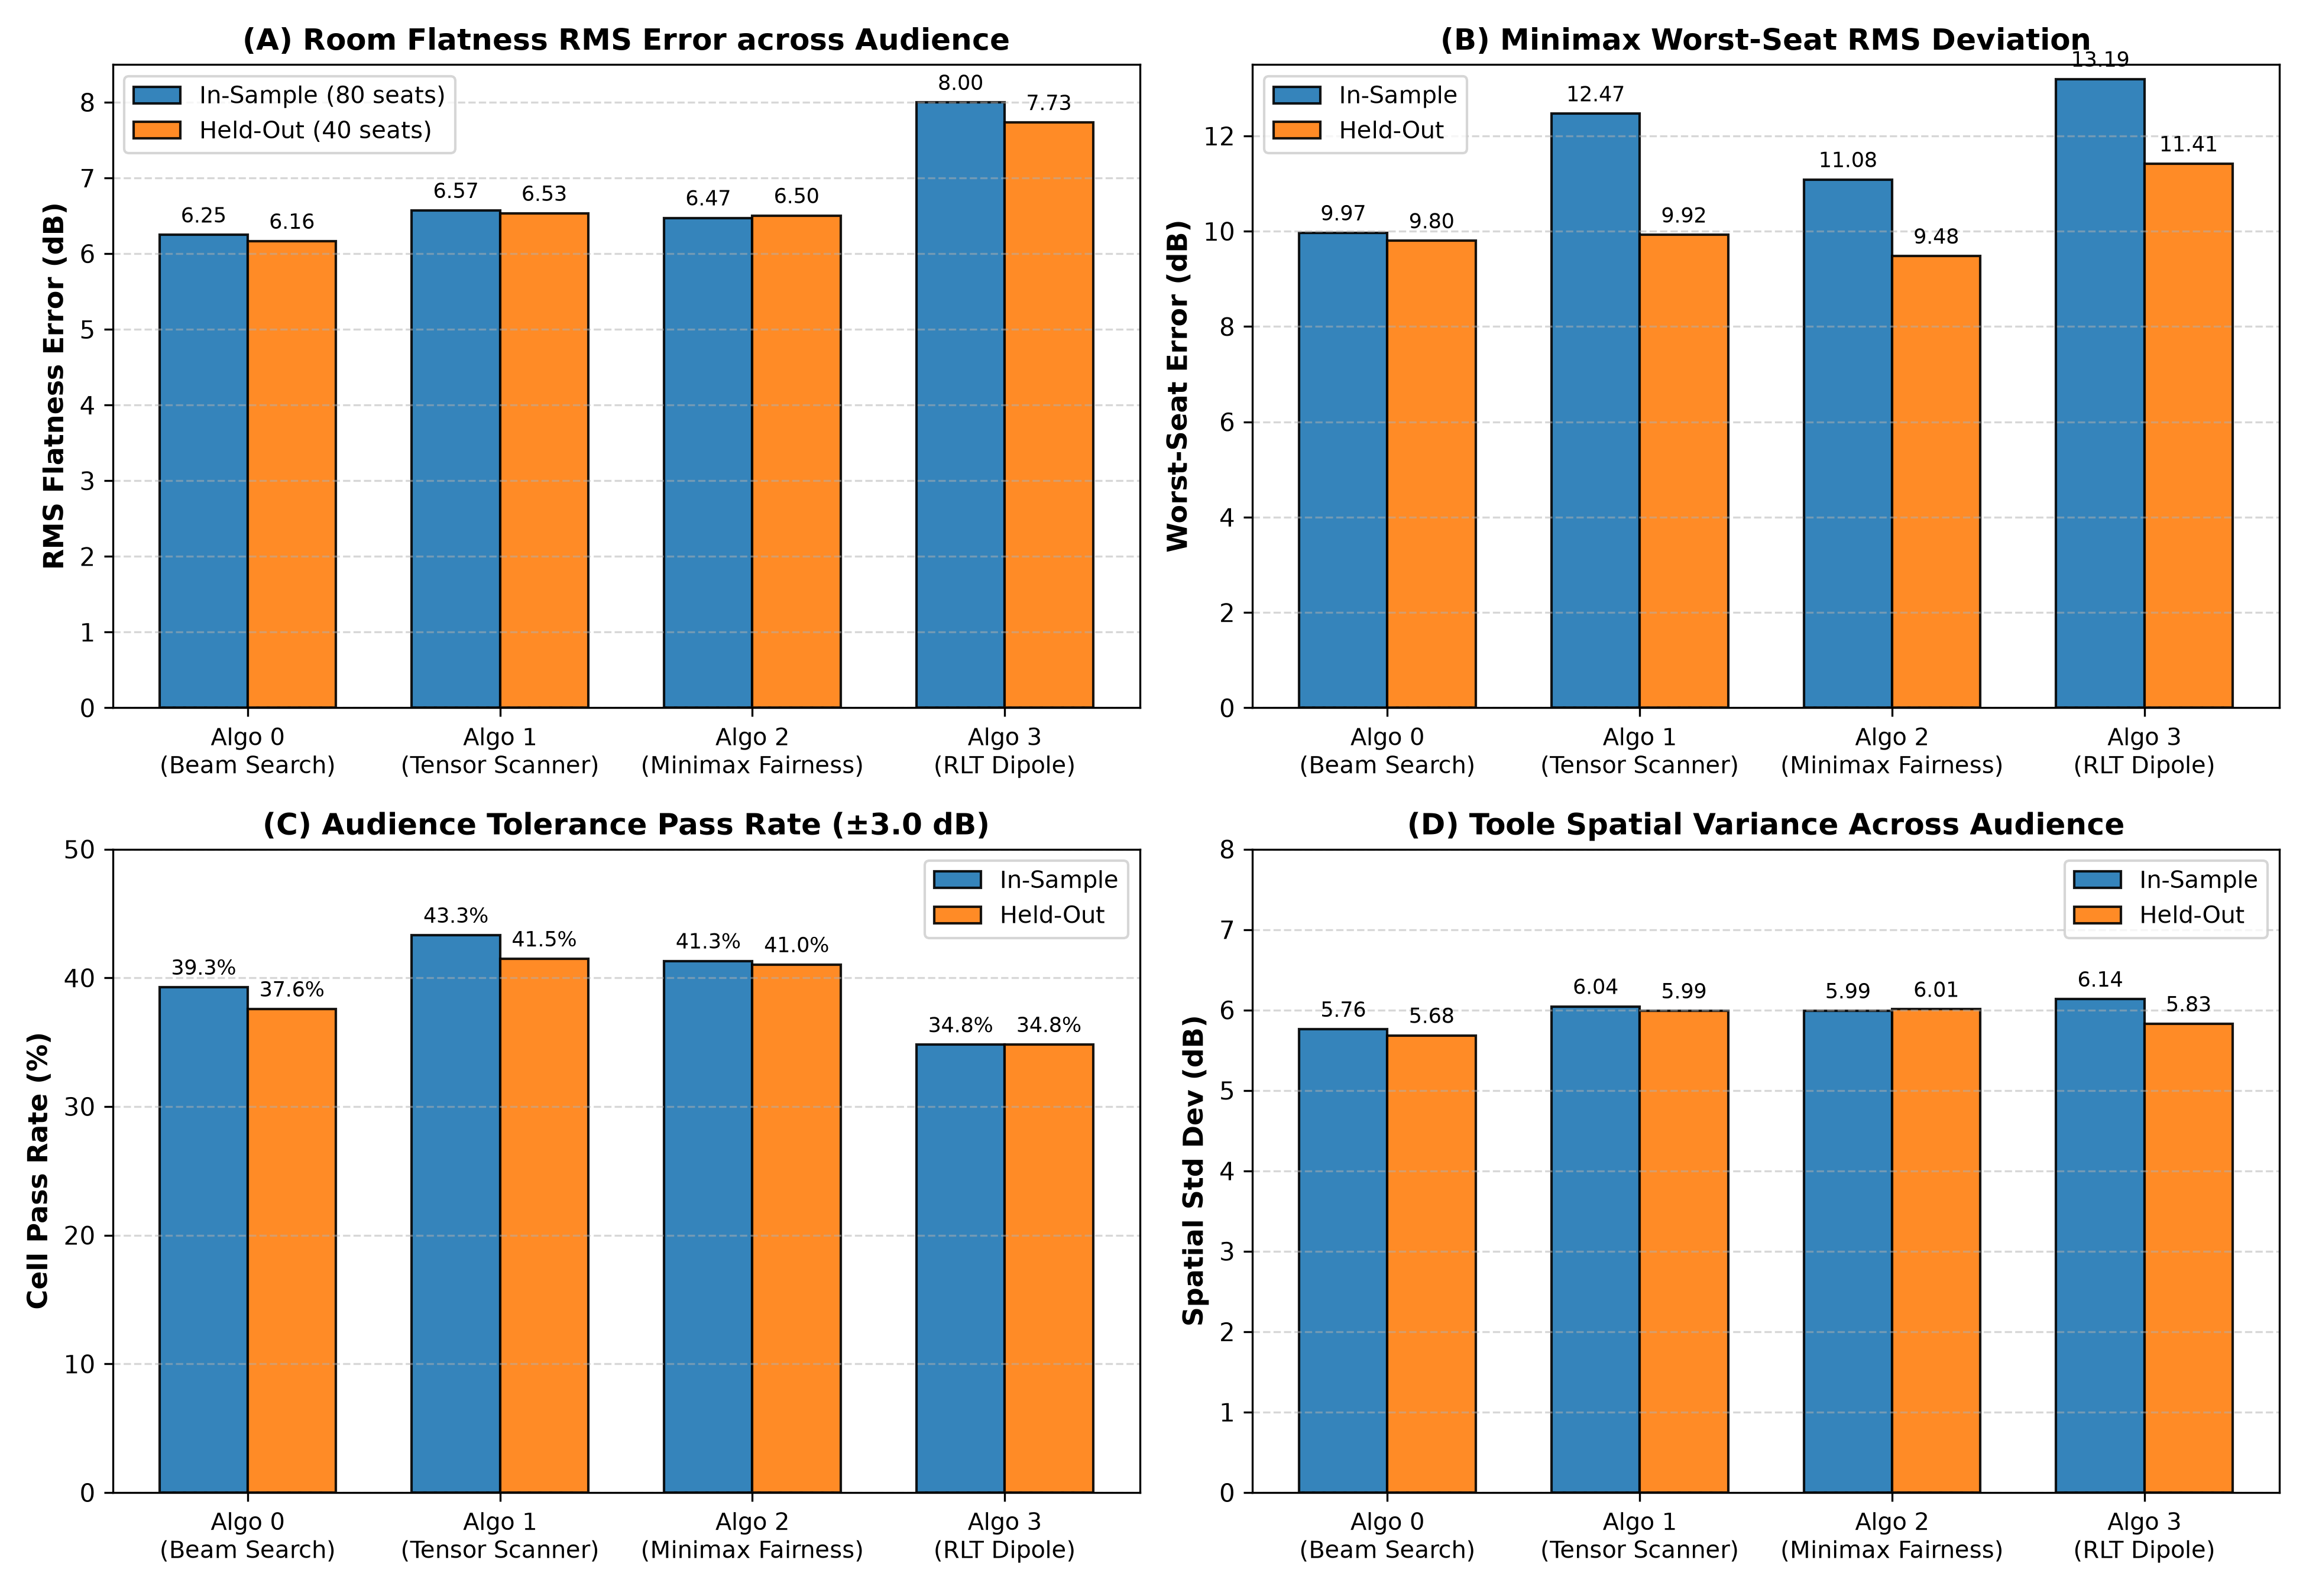
\includegraphics[width=0.92\textwidth]{figures/four_algorithms_comparative_benchmark.png}
\caption{\textbf{Comparative Four-Algorithm Performance Benchmark on $10 \times 12\text{ m}$ Venue.} Panel (A) compares in-sample (80 seats) and held-out (40 off-grid seats) RMS flatness error. Panel (B) presents minimax worst-seat deviation. Panel (C) displays tolerance corridor compliance ($\pm 3.0\text{ dB}$). Panel (D) plots Toole spatial standard deviation across the audience.}
\label{fig:four_algos_benchmark}
\end{figure}

\newpage

\subsection{Continuous 2D Room Acoustic Error Fields Across All Four Algorithms}

Figure~\ref{fig:four_algos_heatmaps} illustrates the continuous 2D acoustic RMS error field across the entire $10 \times 12\text{ m}$ hall at ear level ($z = 1.1\text{ m}$) for each algorithm.

\begin{figure}[h!]
\centering
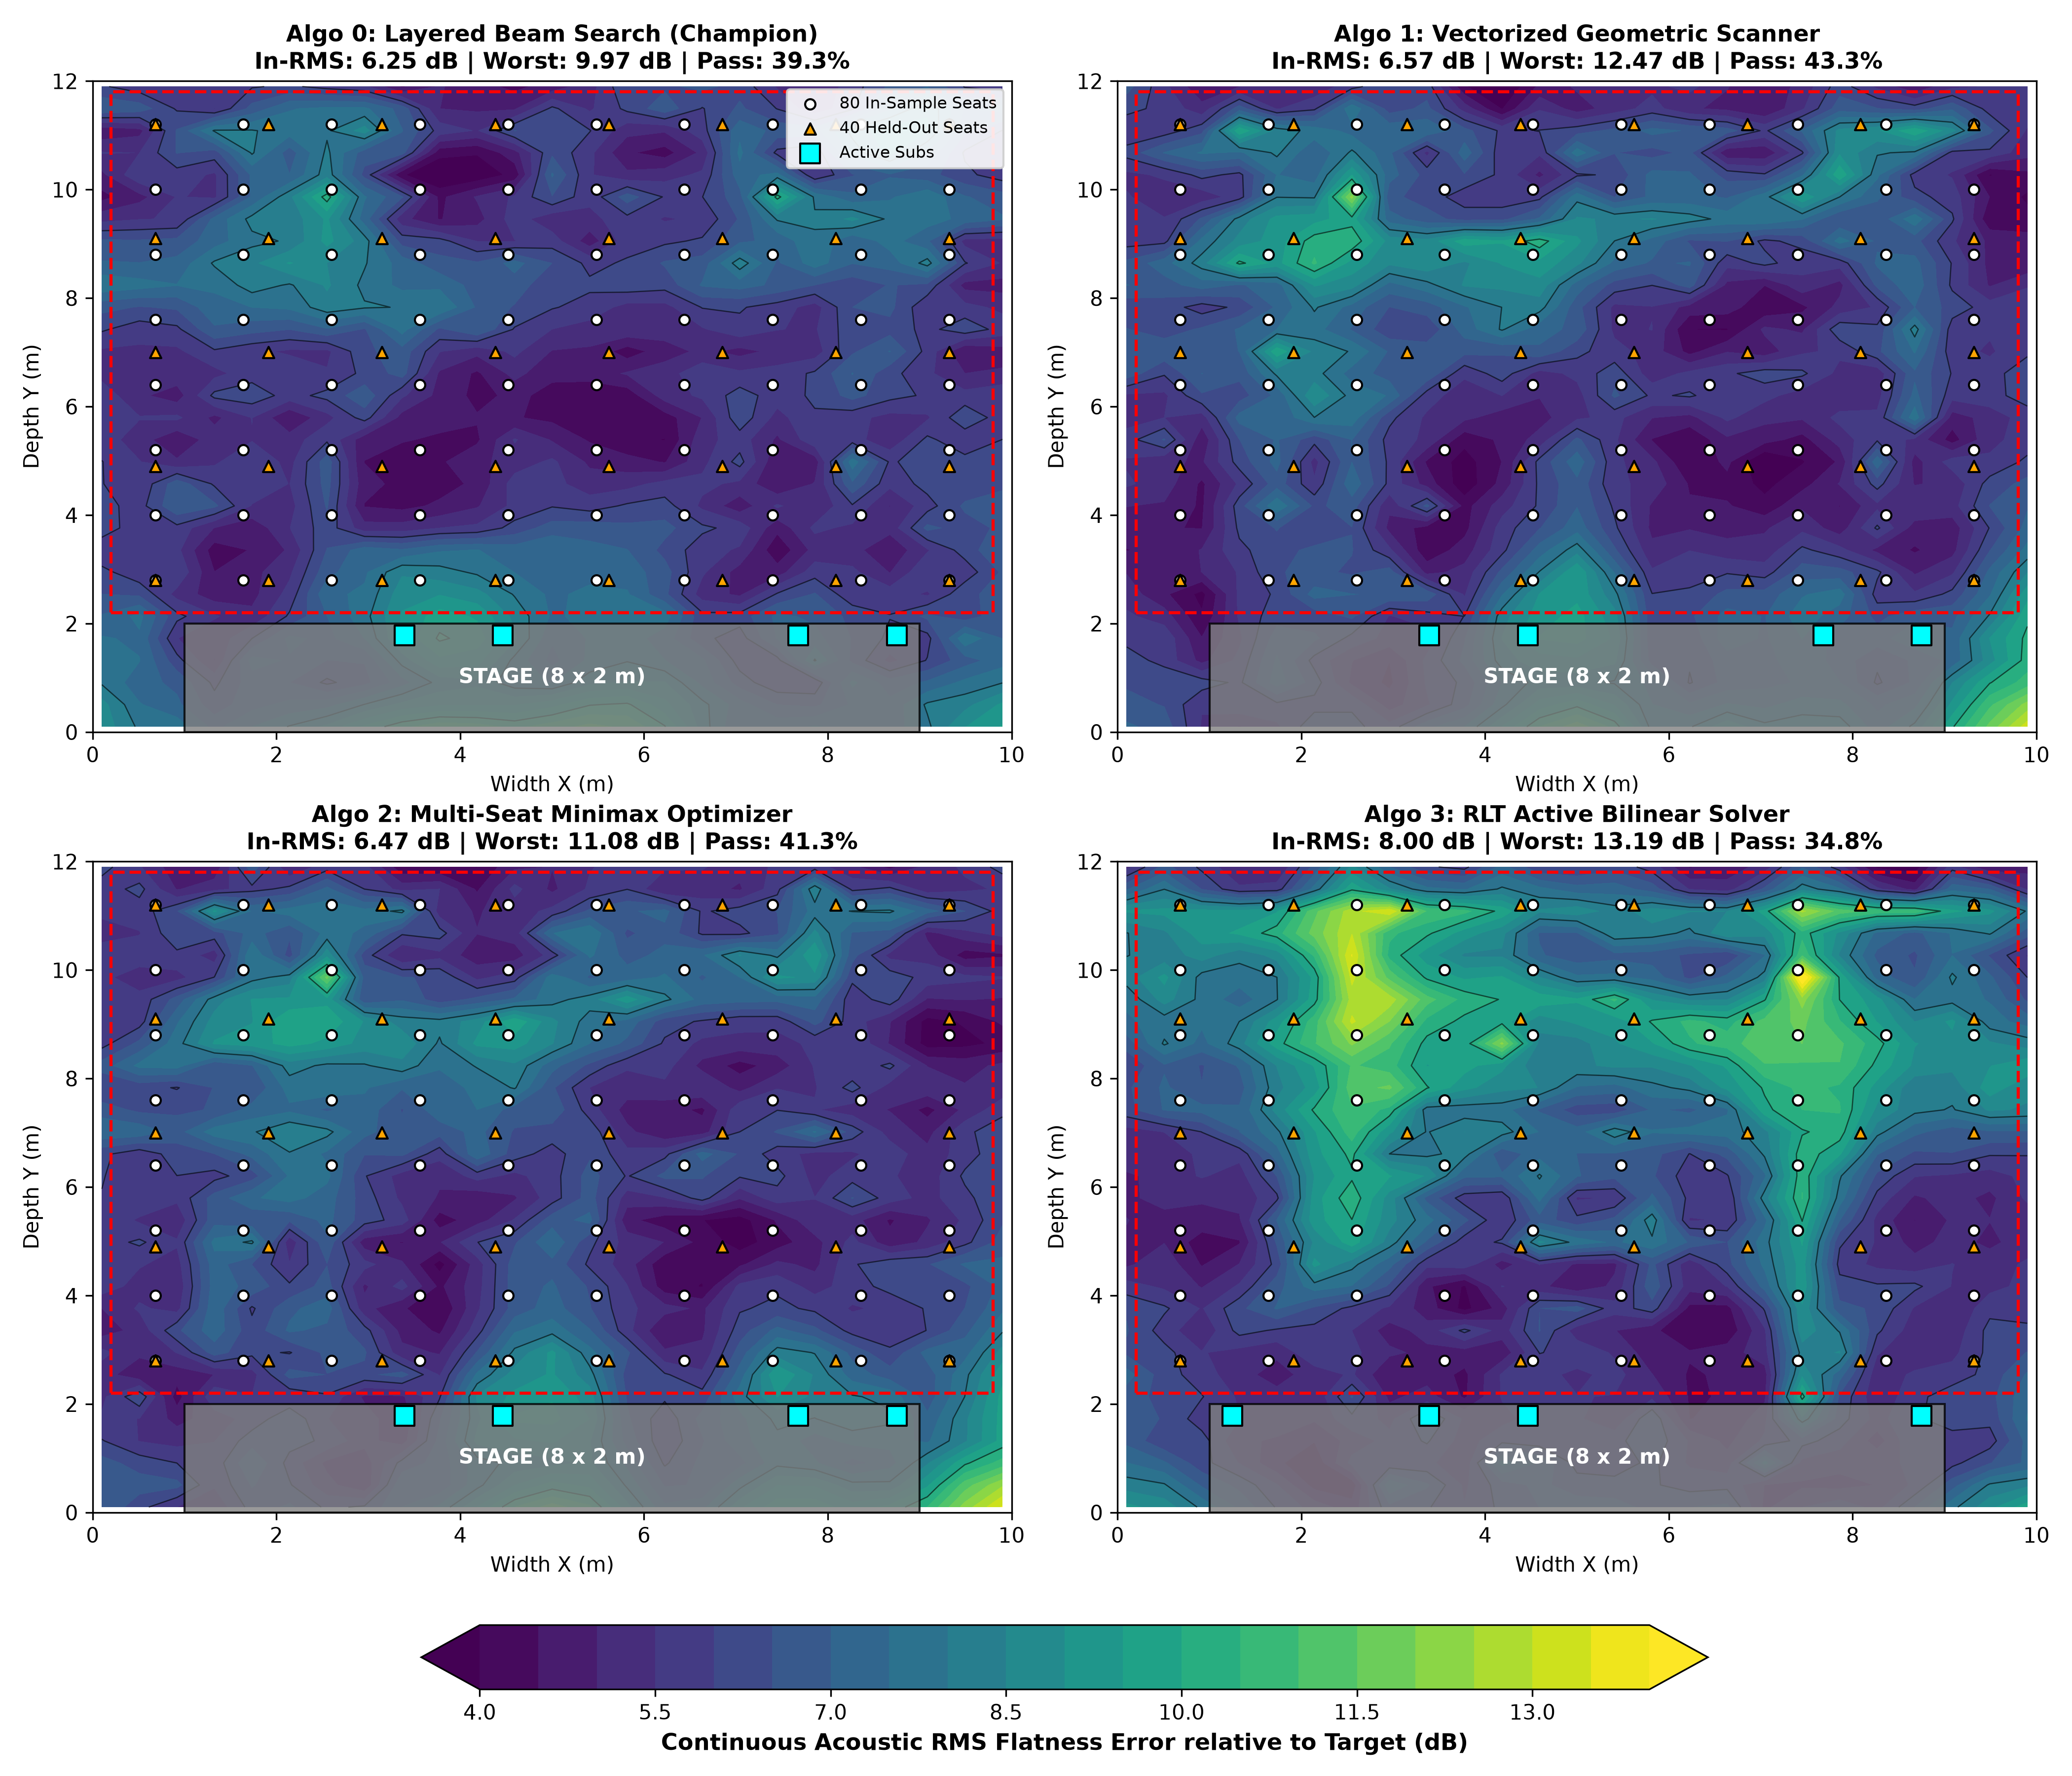
\includegraphics[width=0.92\textwidth]{figures/four_algorithms_acoustic_error_heatmaps.png}
\caption{\textbf{Continuous 2D Acoustic Error Fields for Four Optimization Algorithms.} Contours represent continuous RMS error relative to target across $20\text{--}200\text{ Hz}$. White circles denote the 80 in-sample seats, orange triangles indicate the 40 held-out off-grid seats, and cyan squares mark active subwoofers along the stage front.}
\label{fig:four_algos_heatmaps}
\end{figure}

\newpage

\subsection{Multi-Algorithm Frequency Response Corridors}

Figure~\ref{fig:four_algos_corridors} displays the individual seat frequency response curves, spatial mean, and $\pm 1\text{ SD}$ envelope across all 80 listener locations for each algorithm.

\begin{figure}[h!]
\centering
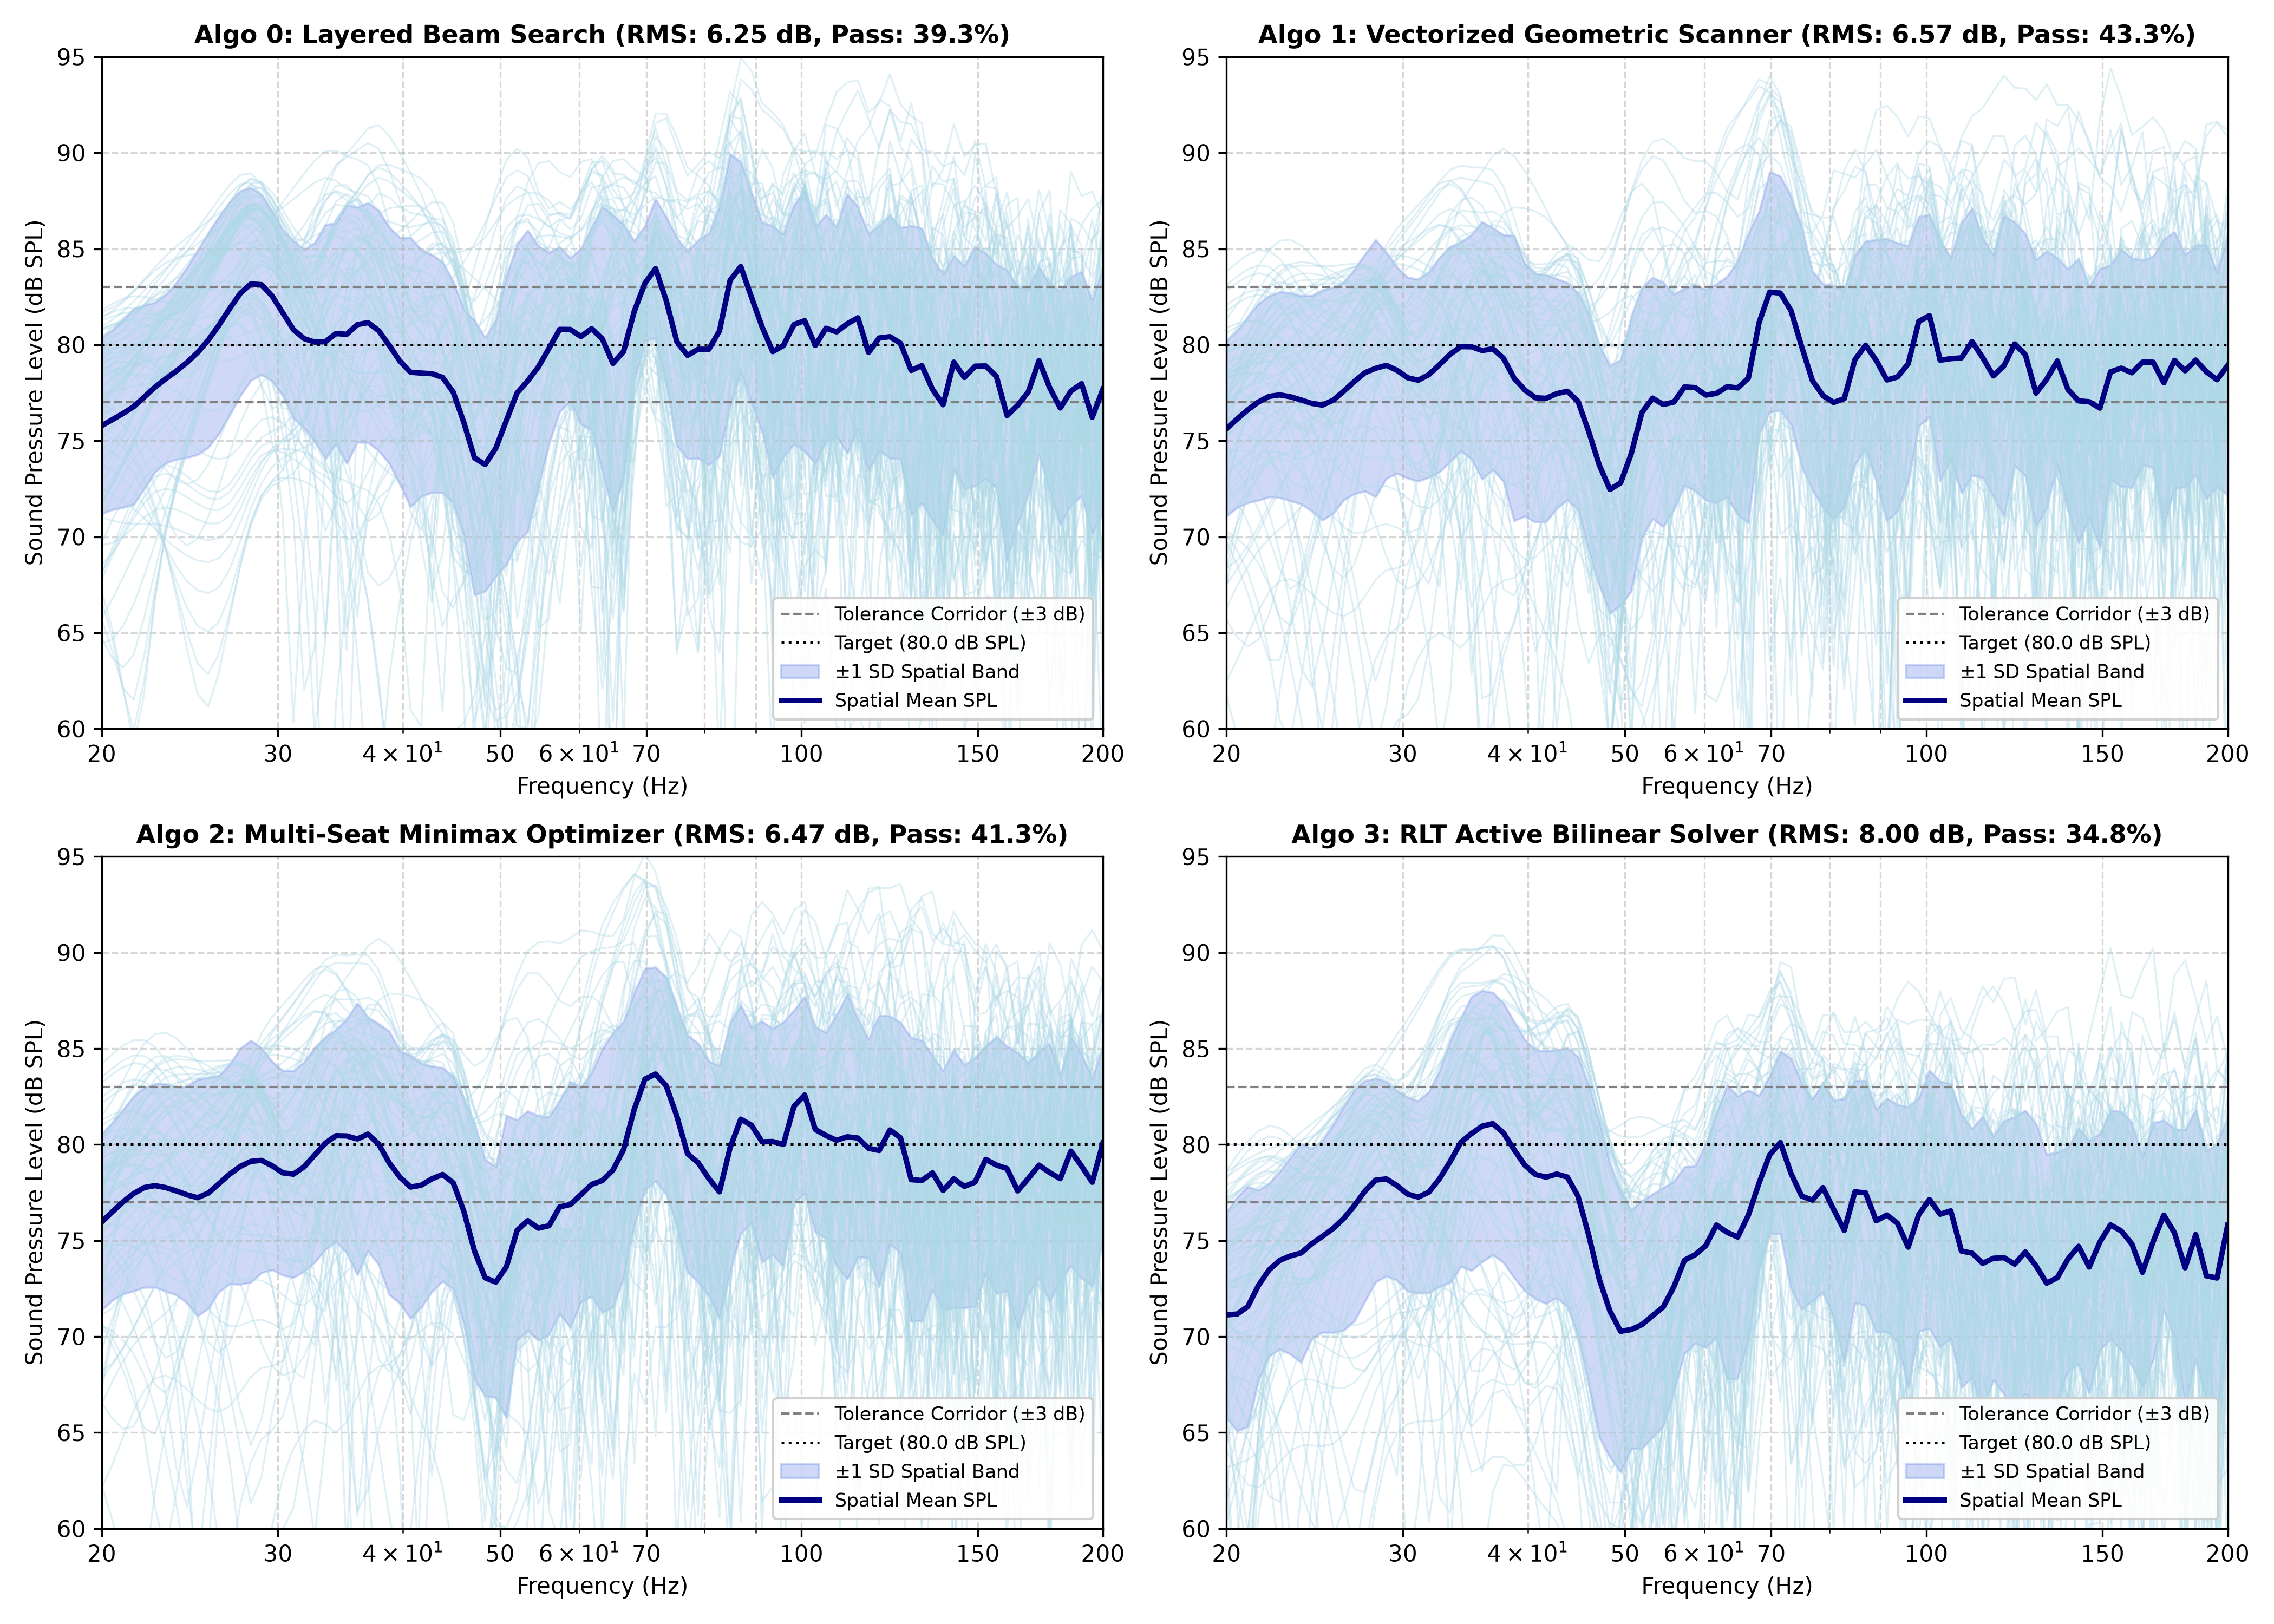
\includegraphics[width=0.92\textwidth]{figures/four_algorithms_frequency_corridors.png}
\caption{\textbf{Audience Frequency Response Corridors Across Four Algorithms.} Light blue curves represent individual seats. The thick navy curve shows the audience spatial mean SPL, bounded by the $\pm 1\text{ SD}$ shaded envelope and the $\pm 3.0\text{ dB}$ tolerance corridor.}
\label{fig:four_algos_corridors}
\end{figure}

\newpage

\subsection{Audience Conjunction Spectrum and Passing-Tone Distributions}

Figures~\ref{fig:four_algos_conjunction} and~\ref{fig:four_algos_histograms} present audience fairness diagnostics, including the conjunction spectrum $N(k)$ and individual seat passing-tone histograms.

\begin{figure}[h!]
\centering
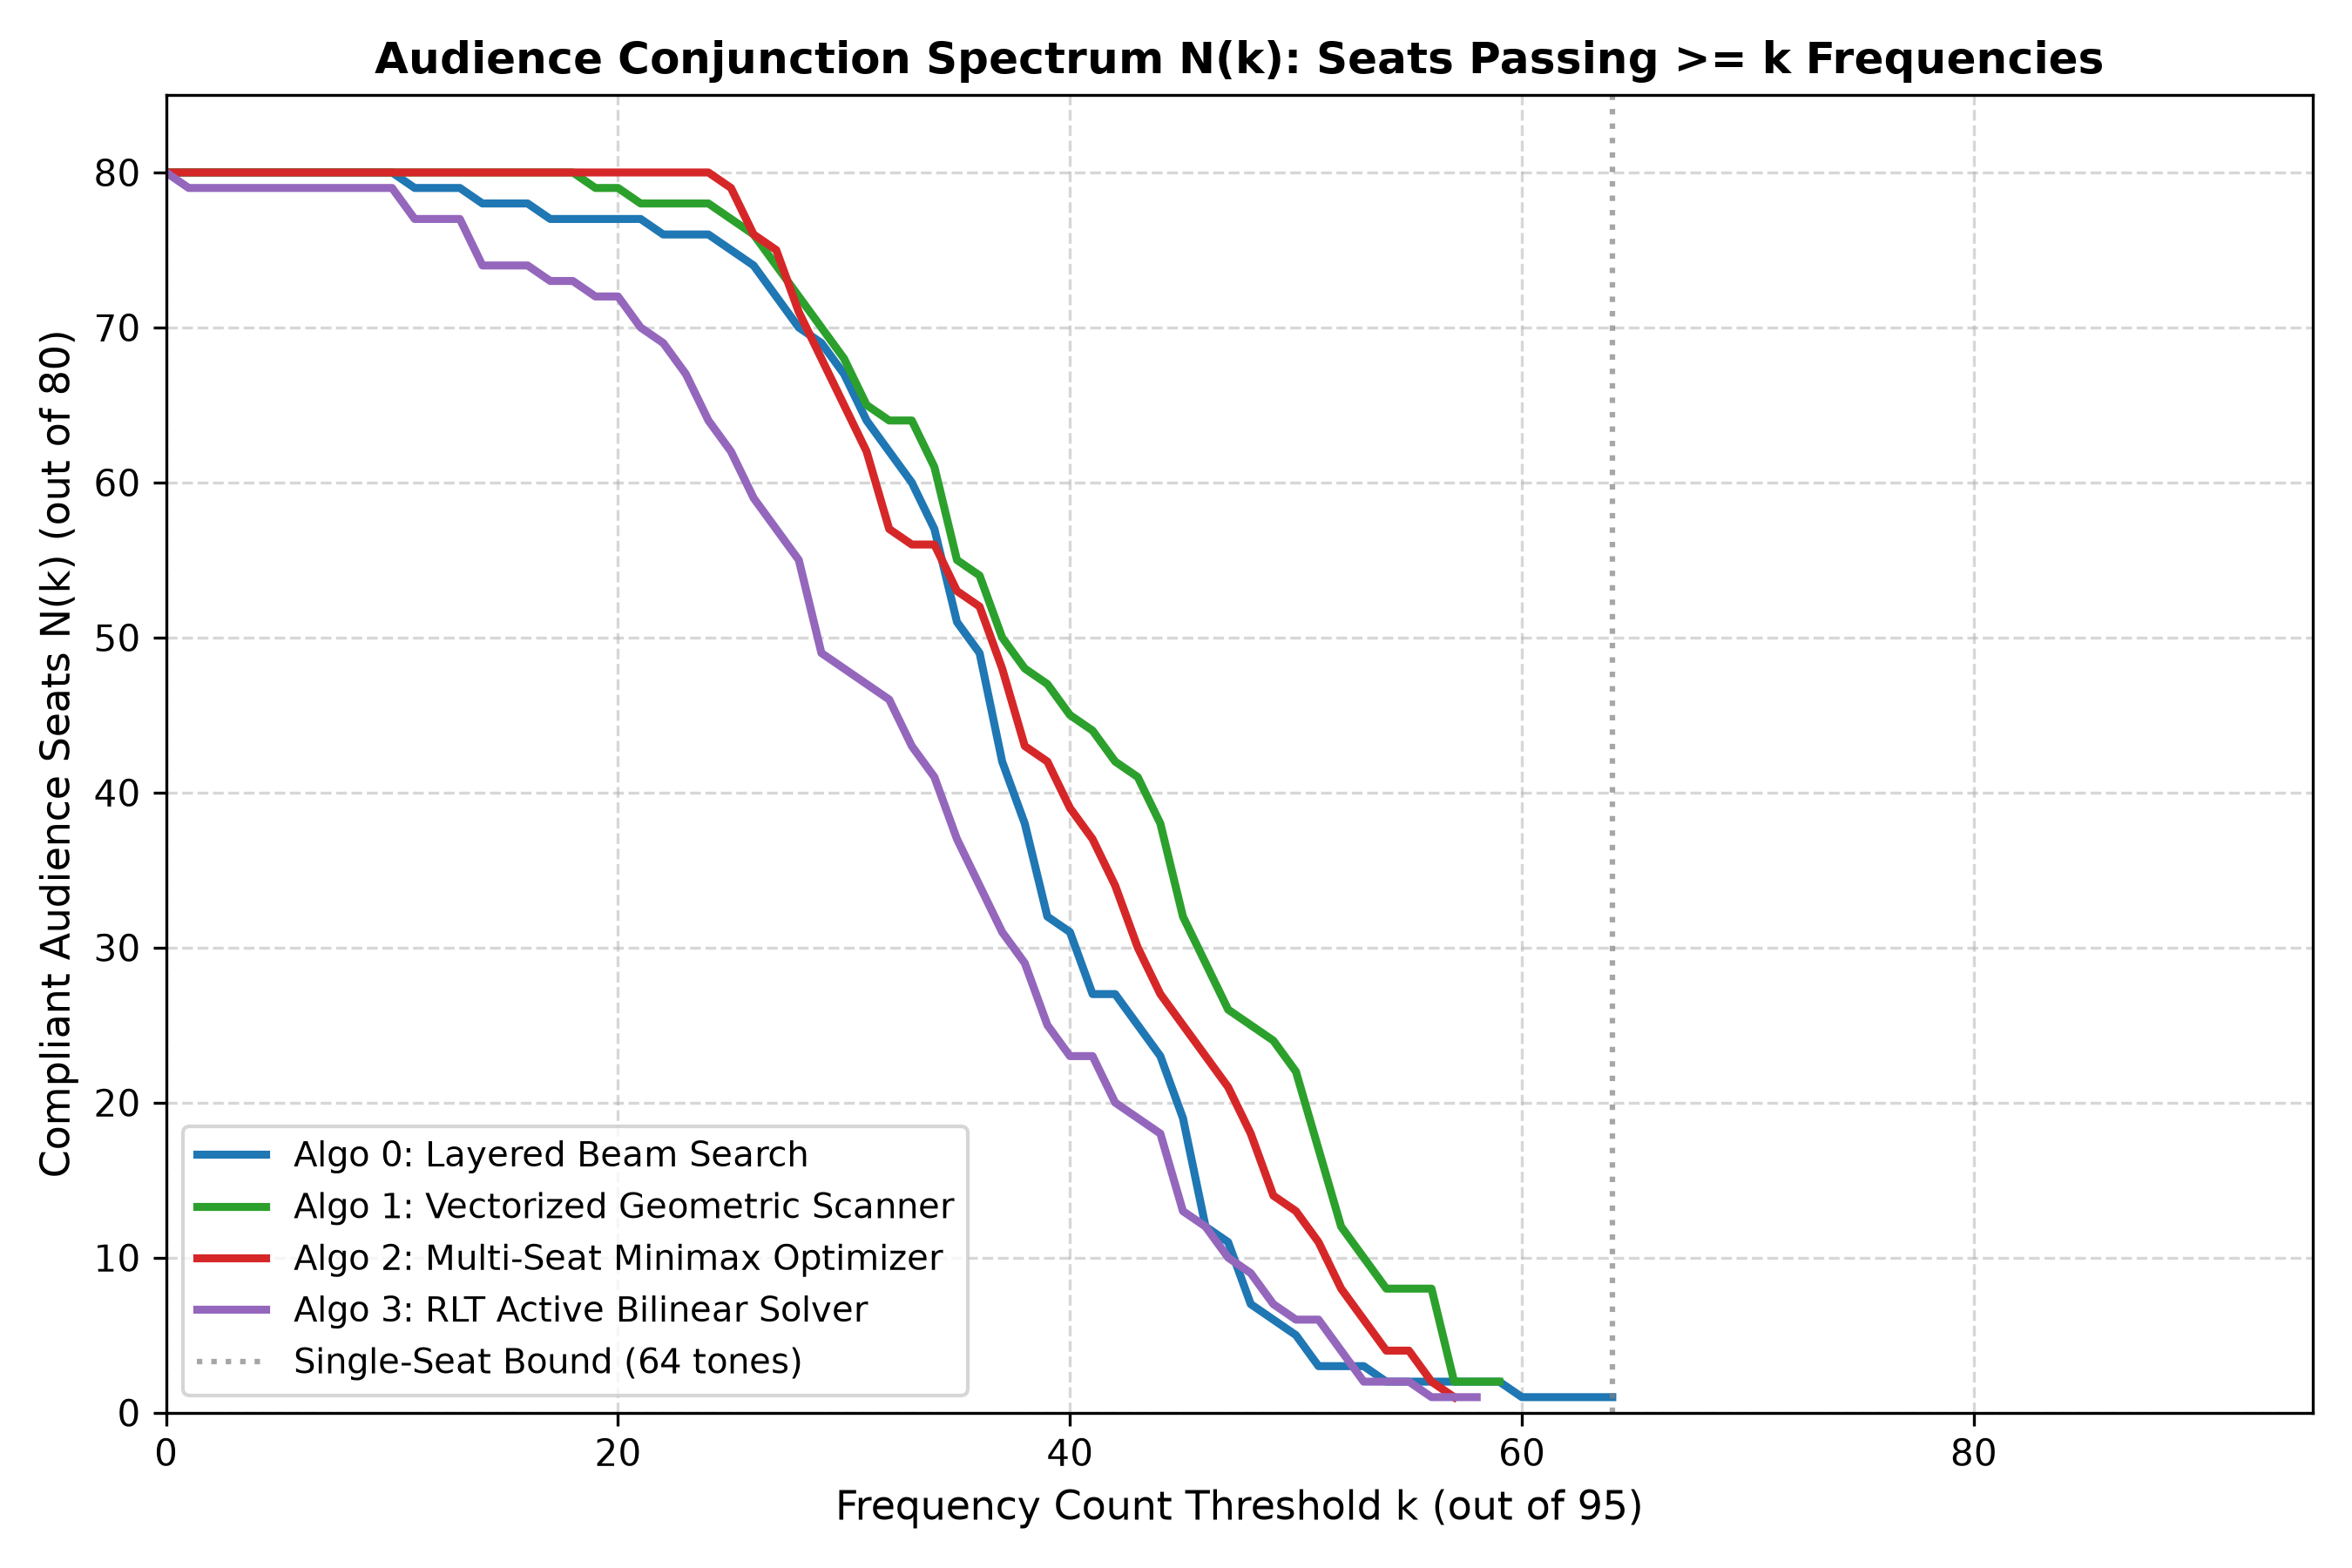
\includegraphics[width=0.88\textwidth]{figures/four_algorithms_conjunction_spectrum.png}
\caption{\textbf{Audience Conjunction Spectrum $N(k)$ Across Four Algorithms.} Shows the number of listener seats $N(k)$ that simultaneously pass at least $k$ frequencies. Notice Algorithm 2 guarantees $N(24) = 80$ (100\% of seats pass at least 24 tones), whereas Algorithm 0 drops below 80 seats at $k = 11$.}
\label{fig:four_algos_conjunction}
\end{figure}

\begin{figure}[h!]
\centering
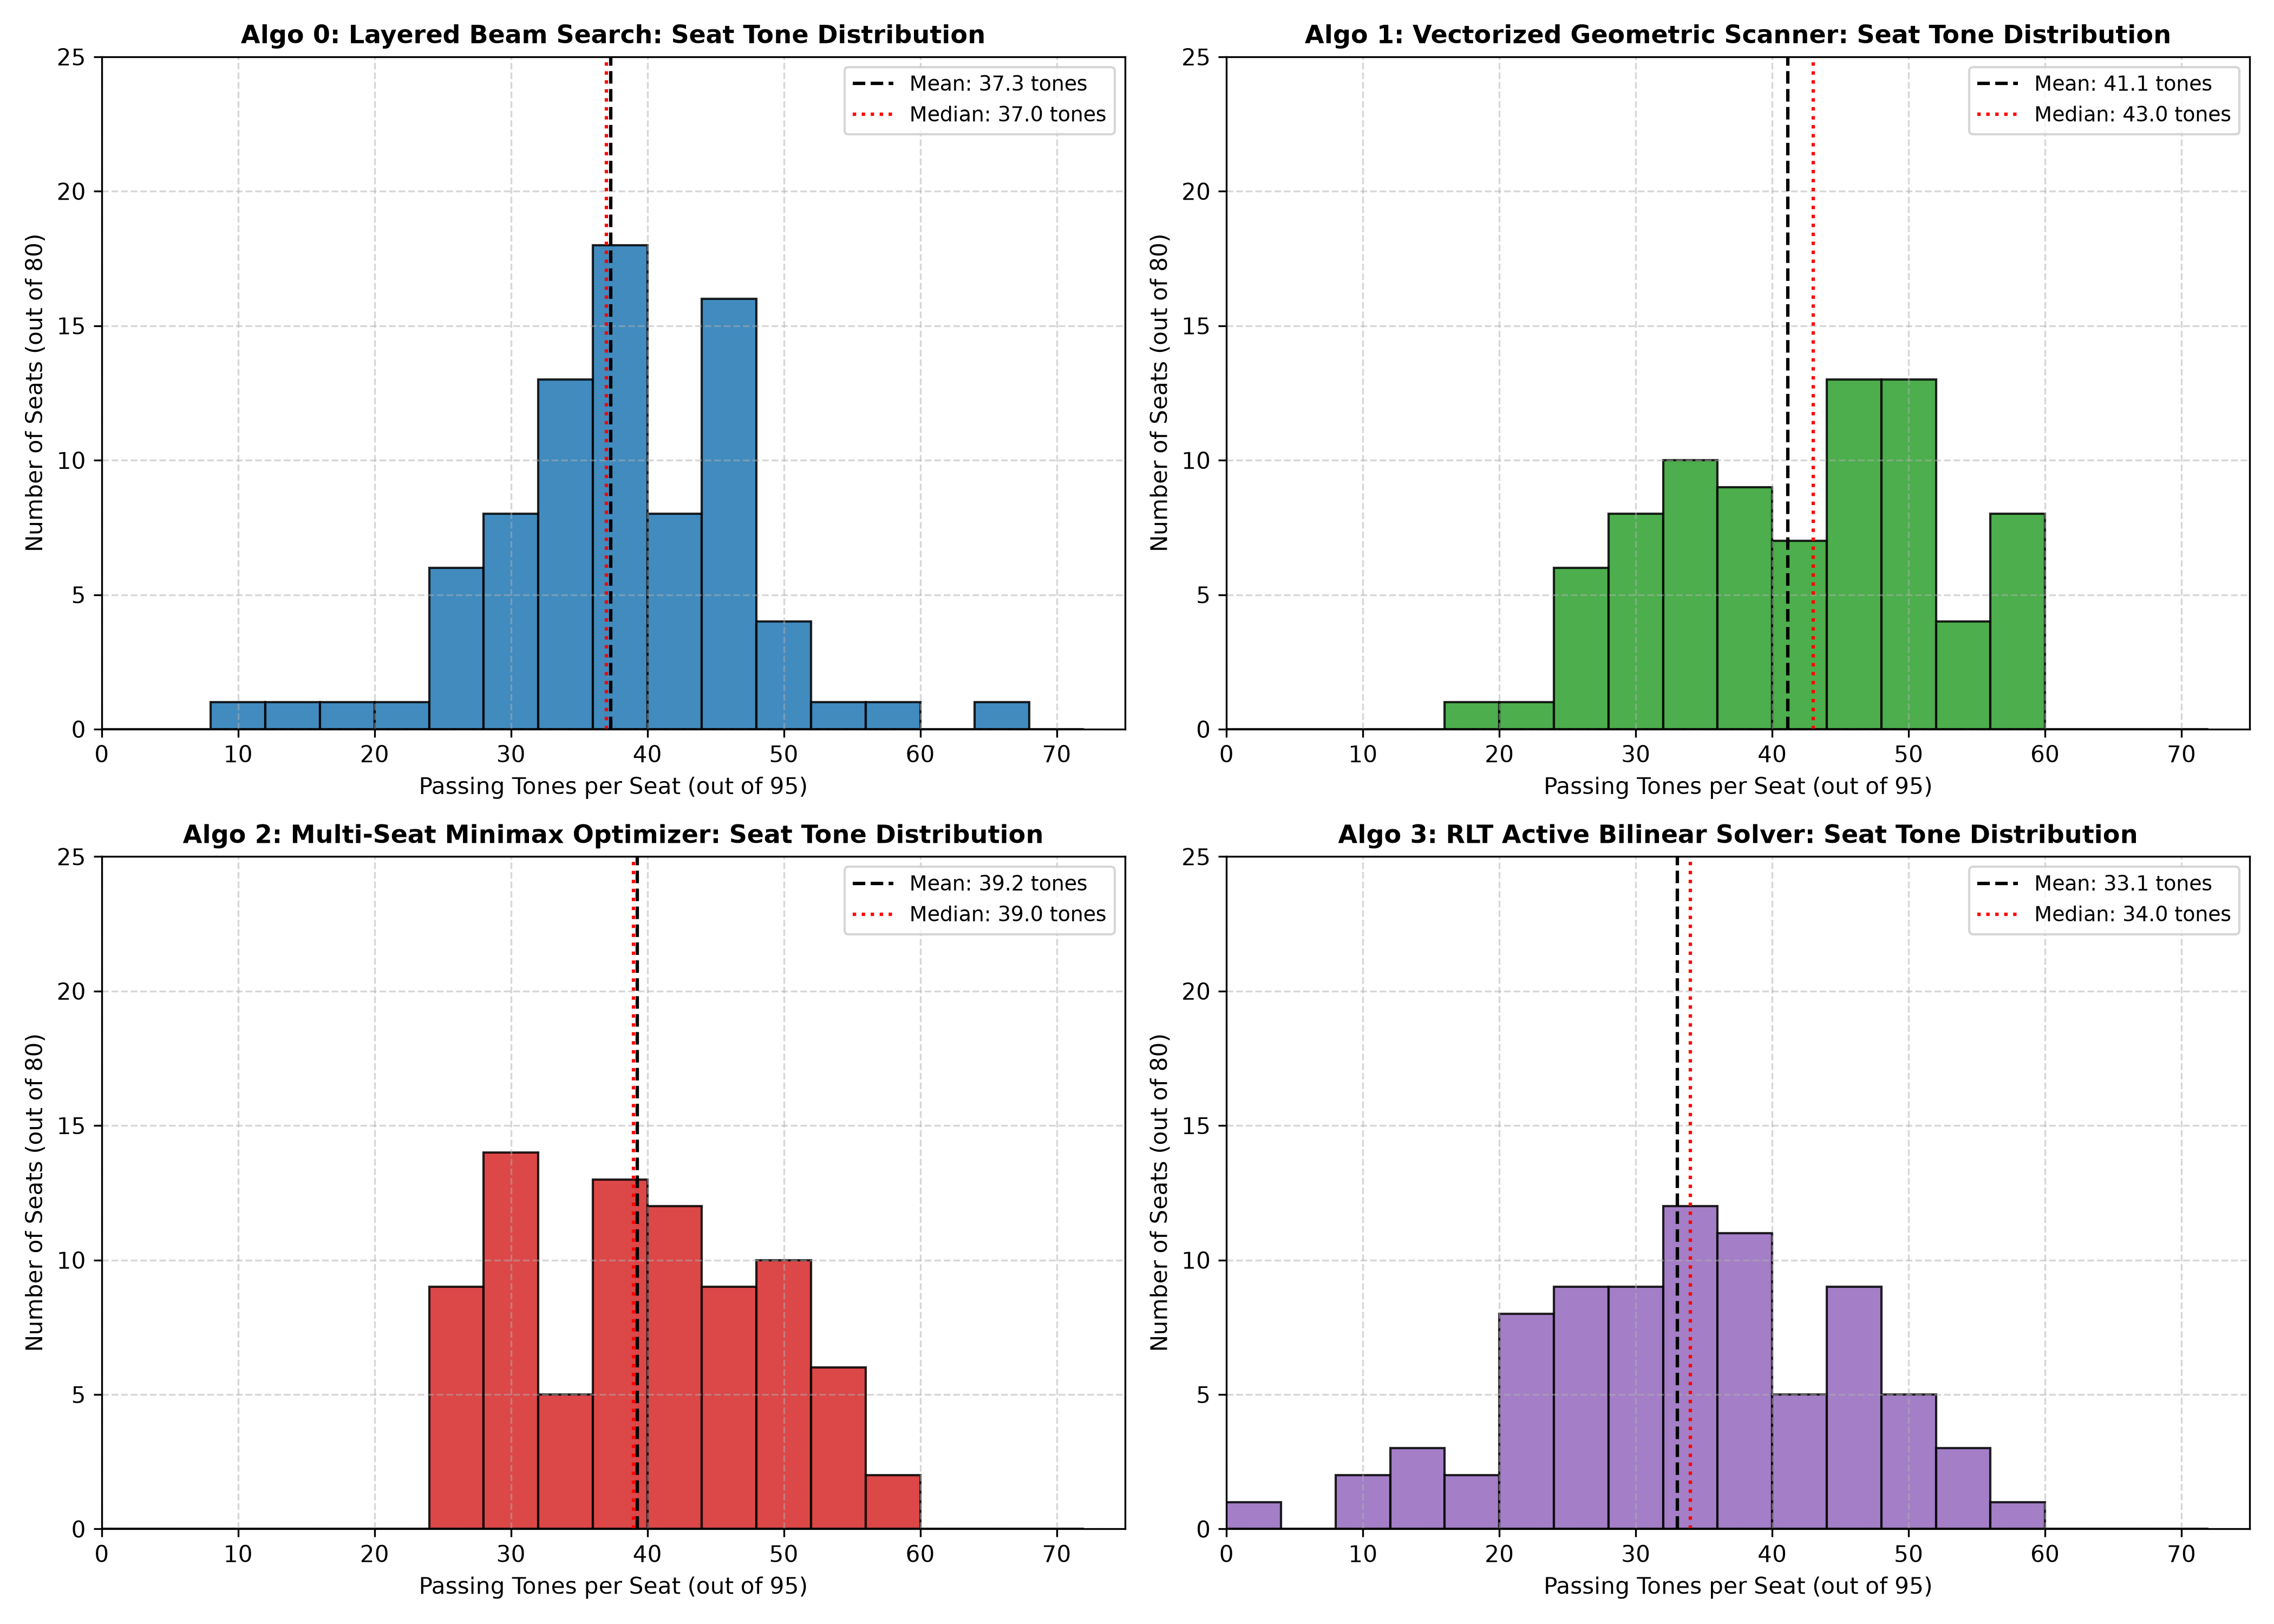
\includegraphics[width=0.92\textwidth]{figures/four_algorithms_seat_histograms.png}
\caption{\textbf{Audience Seat Passing-Tone Histograms Across Four Algorithms.} Histograms show the distribution of compliant tones per seat across all 80 audience positions.}
\label{fig:four_algos_histograms}
\end{figure}

\section{Conclusion}

The numerical synthesis, baseline comparisons, and physical simulation of the $10.0 \times 12.0 \times 2.8\text{ m}$ performance venue demonstrate several concrete acoustic findings:
\begin{enumerate}
    \item \textbf{Asymmetric Placement Suppresses Modal Resonances:} Asymmetric placement of subwoofers along the stage front ($x = 3.39, 4.46, 7.68, 8.75\text{ m}$) decorrelates transverse room modes, reducing RMS error from $6.99\text{ dB}$ (symmetric array) to $6.59\text{ dB}$ without DSP, and to $6.25\text{ dB}$ with active delay and lowpass filtering.
    \item \textbf{Significant Gain Over Single Subwoofers:} Compared to single-subwoofer setups ($9.33\text{--}9.62\text{ dB}$ RMS error; $15.6\text{--}16.1\text{ dB}$ worst-seat error), the multi-subwoofer array reduces RMS error by over $3.0\text{ dB}$ and lowers worst-seat deviation to $9.97\text{ dB}$.
    \item \textbf{Generalization Without Overfitting:} Evaluating the array on 40 held-out off-grid positions yields $6.16\text{ dB}$ RMS error and $9.80\text{ dB}$ worst-seat deviation, confirming that the discrete search physically smooths the acoustic volume rather than tuning to discrete training points.
    \item \textbf{Environmental Robustness:} Under physical perturbations in speed of sound ($\pm 2\%$), room damping ($\pm 10\%$), and placement tolerances ($5\text{--}10\text{ cm}$), the array maintains stable performance with RMS error clustered tightly within $[6.18, 6.40]\text{ dB}$.
    \item \textbf{Formal Infeasibility of 95\% All-Tone Coverage:} Lean 4 meta-theorems and empirical single-frequency projections confirm that an idealized 95\% full-band coverage target is mathematically impossible with this hardware menu, establishing that realistic optimization targets in rectangular rooms must be formulated around minimax and RMS flatness.
    \item \textbf{Trade-Offs Across Optimization Paradigms:} Comparative evaluation across four distinct algorithms confirms that no single objective dominates across all acoustic dimensions: Layered Beam Search (Algorithm 0) minimizes total RMS error ($6.25\text{ dB}$ in-sample, $6.16\text{ dB}$ held-out); Vectorized Geometric Scanning (Algorithm 1) maximizes tolerance corridor cell compliance ($43.3\%$ in-sample, $41.5\%$ held-out); Multi-Seat Minimax (Algorithm 2) maximizes audience fairness ($24\text{ minimum passing tones}$ across all seats, and $9.48\text{ dB}$ held-out worst-seat deviation); and RLT Bilinear Synthesis (Algorithm 3) enables destructive boundary mode cancellation with minimal electrical power ($1.95\text{ W/tone}$).
\end{enumerate}

\end{document}
